\chapter{Results and Interpretation}

\begin{section}{Examination of Pre-fit Data}
\label{sec:prefit_data}

Before proceeding with the full maximum likelihood fit using all the analysis bins, it is helpful to evaluate the observed, pre-fit data distributions.
The pre-fit \Nb distributions for the control region bins are those shown in Figure~\ref{fig:prefit_cr} and have corresponding yields given in Table~\ref{tab:prefit_cr}, while those for the signal region bins are shown in Figure~\ref{fig:prefit_sr} and Table~\ref{tab:prefit_sr}.
In Figure~\ref{fig:prefit_cr} and Figure~\ref{fig:prefit_sr}, the background normalization is scaled to match the observed data yields in each bin with a scaling factor that controls all processes equally.
This approximates the effect of the various normalization parameters in the fit and allows for a rough comparison of the background and observed \Nb distribution shapes.
By examining this comparison, a qualitiative understanding of the results and expected fit behavior can be gained.

\begin{figure}[tbp!]
\centering
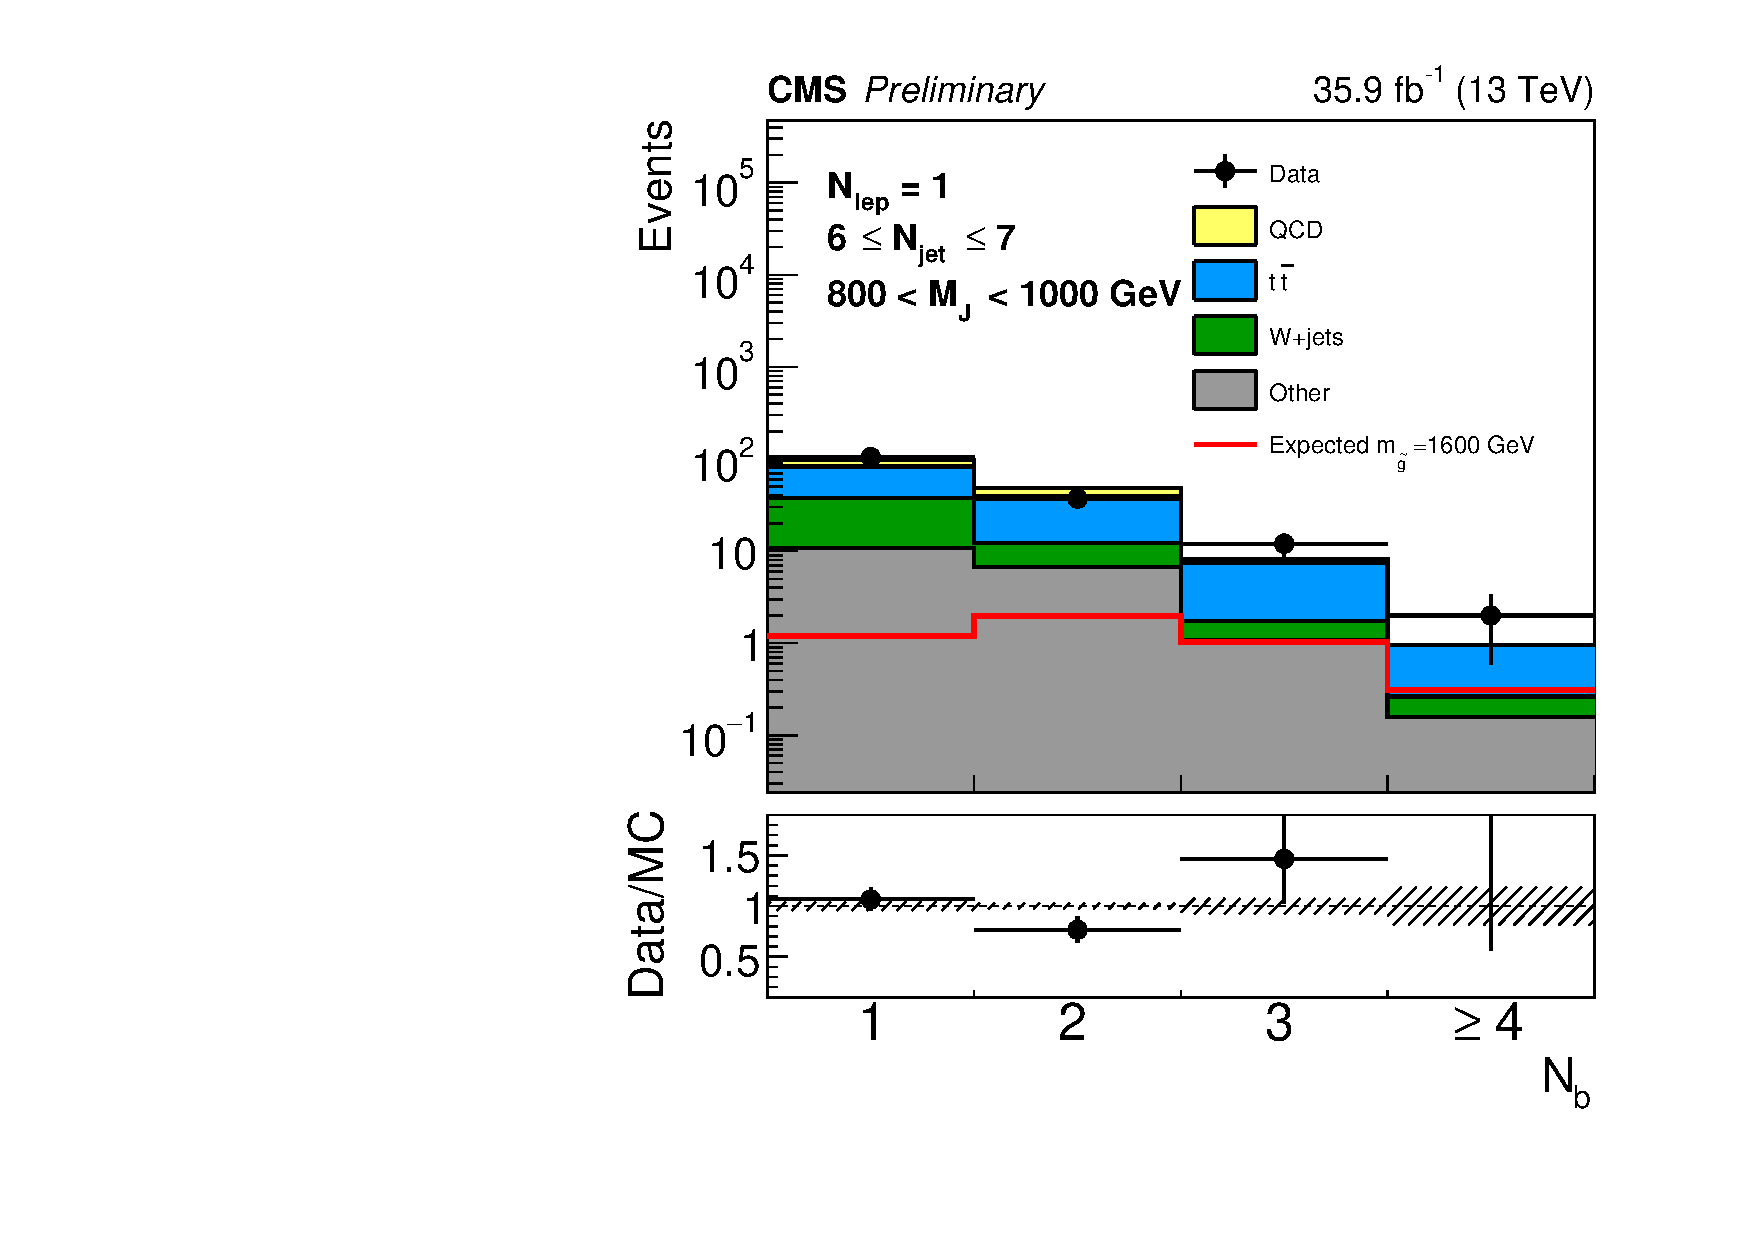
\includegraphics[angle=0,width=0.32\columnwidth]{fig/prefit_nlep1_nj67_highmj.pdf}
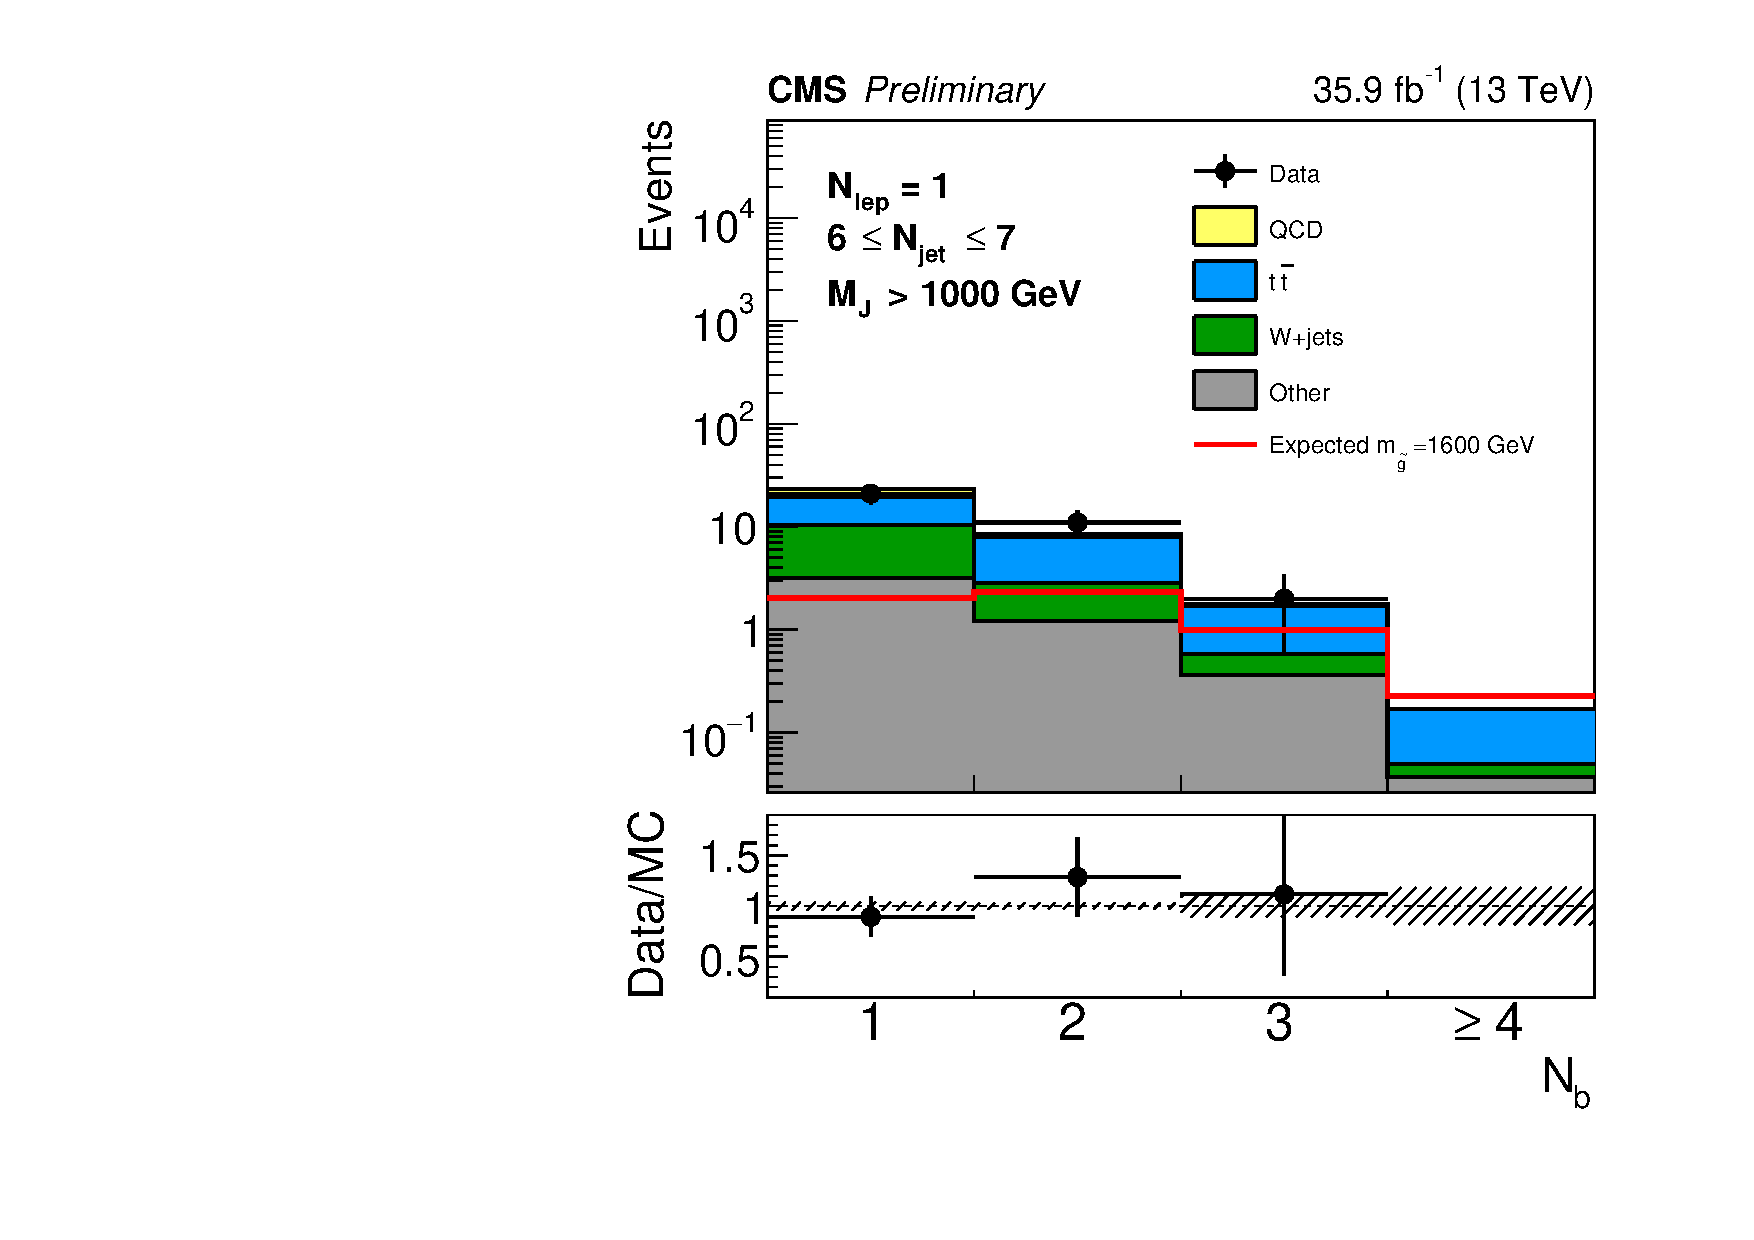
\includegraphics[angle=0,width=0.32\columnwidth]{fig/prefit_nlep1_nj67_vhighmj.pdf}
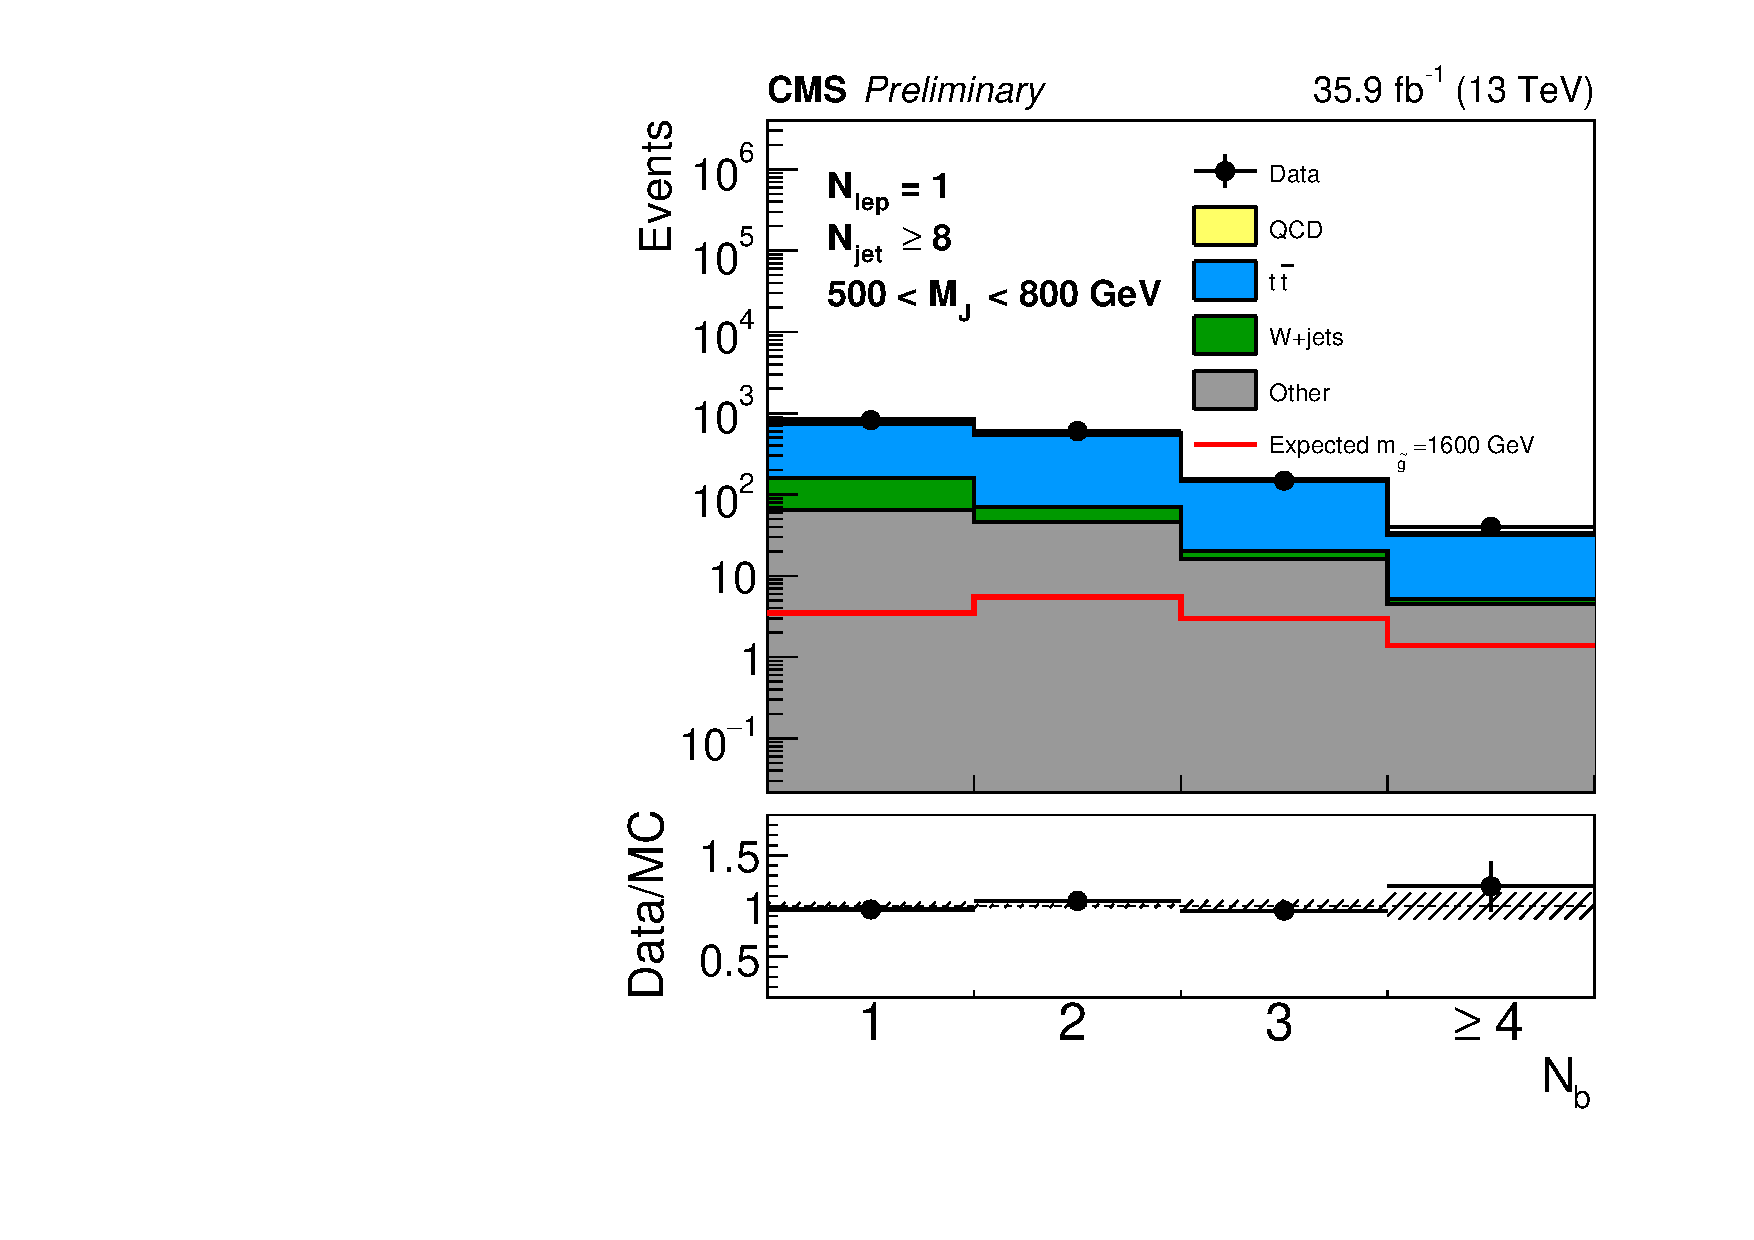
\includegraphics[angle=0,width=0.32\columnwidth]{fig/prefit_nlep1_nj8_lowmj.pdf}
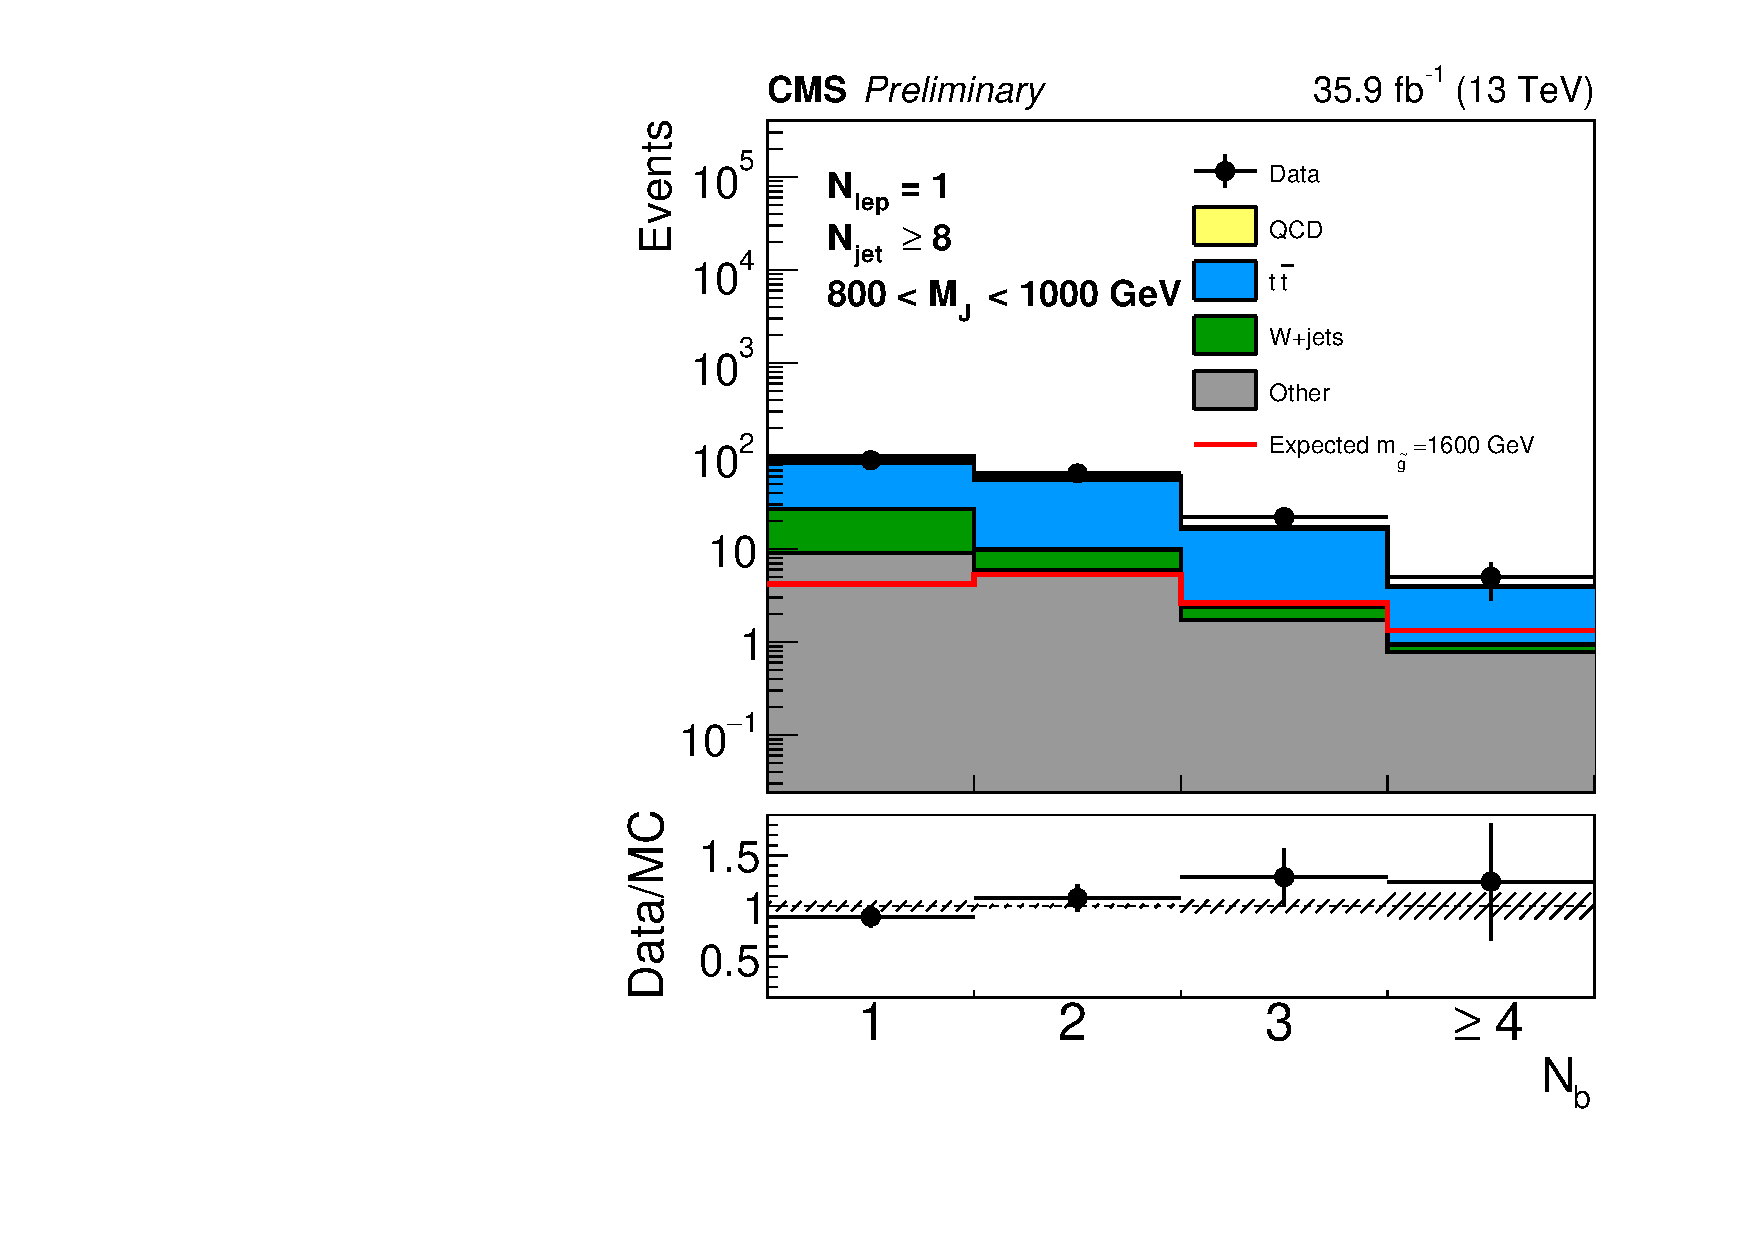
\includegraphics[angle=0,width=0.32\columnwidth]{fig/prefit_nlep1_nj8_highmj.pdf}
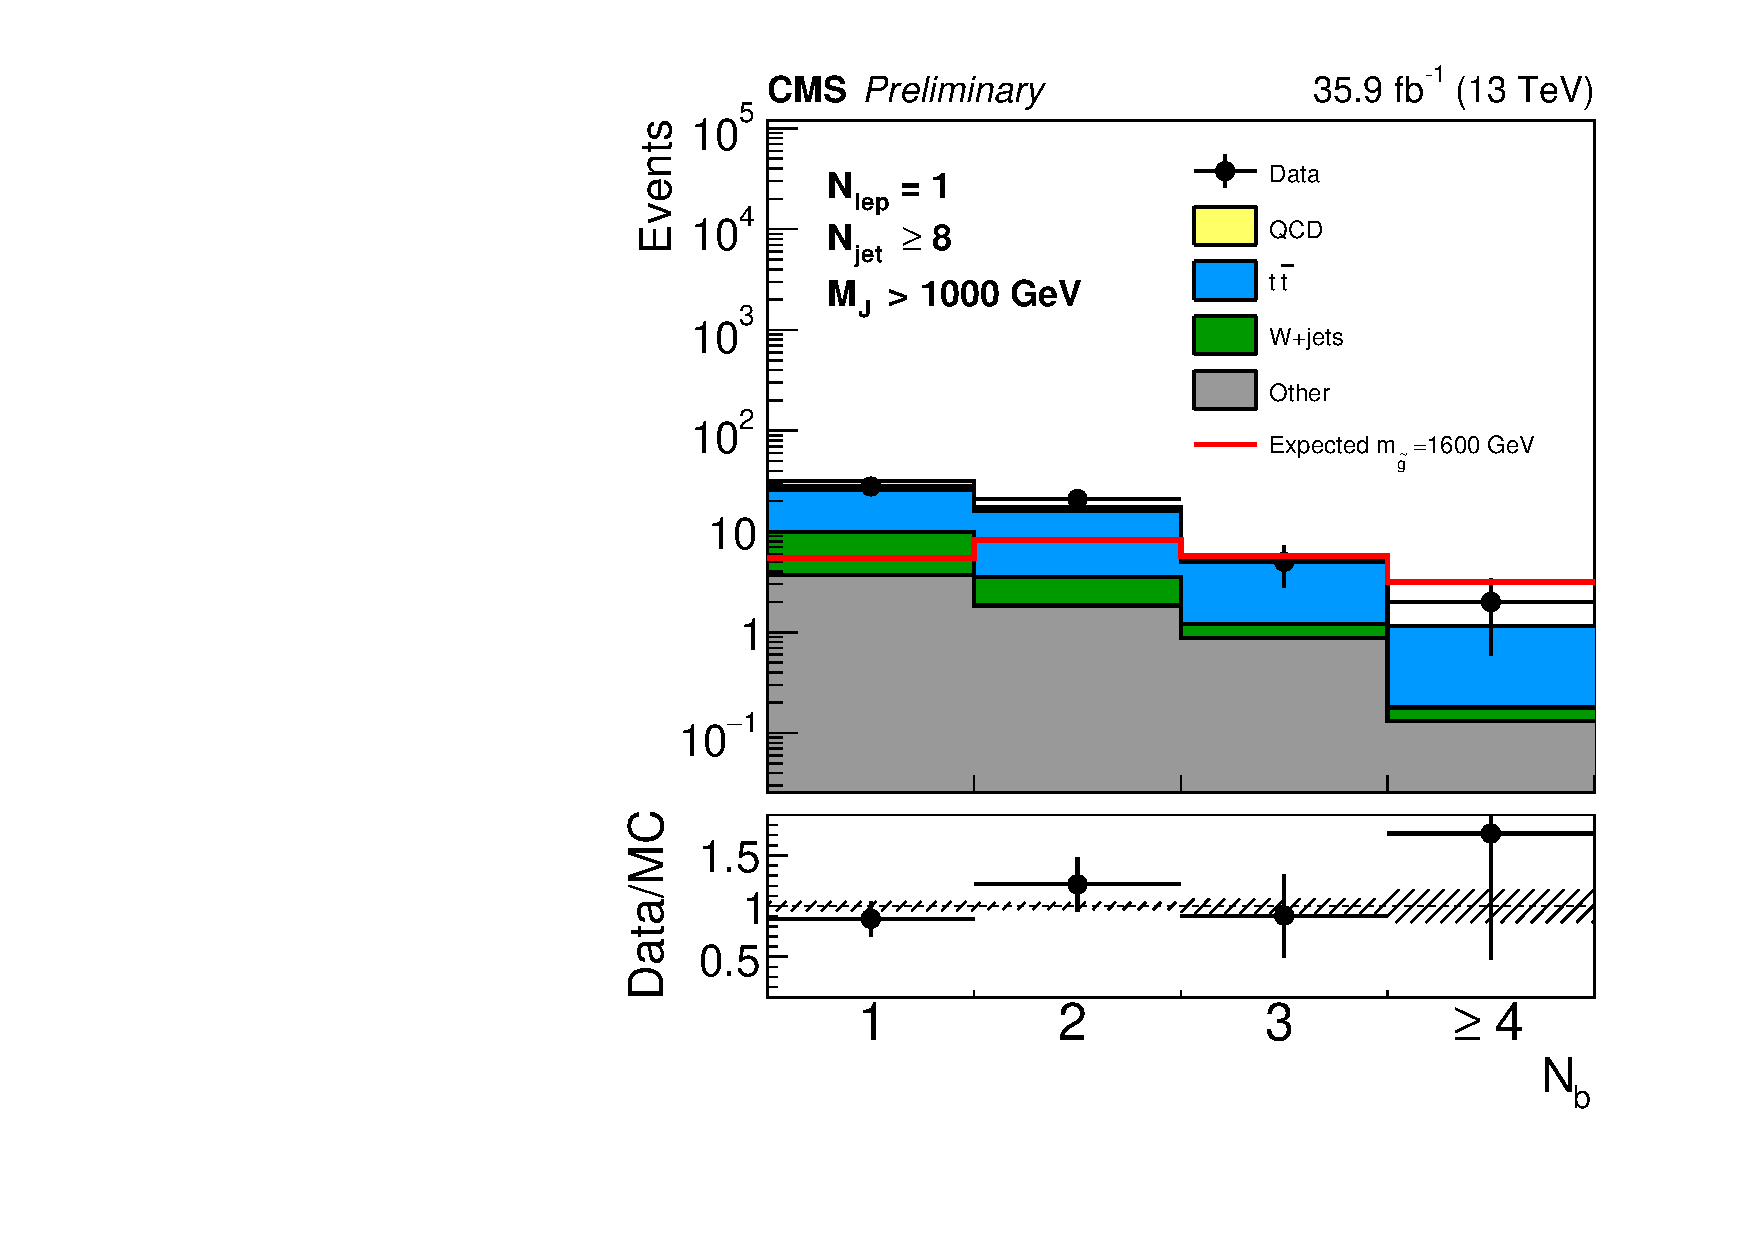
\includegraphics[angle=0,width=0.32\columnwidth]{fig/prefit_nlep1_nj8_vhighmj.pdf}
\caption{Pre-fit \Nb distributions of the signal region bins with the background simulation normalized to the observed data yields with a single scaling factor: $6 \leq \Njets \leq 7$, $800 < \MJ \leq 1000~\GeV$ (upper-left), $6 \leq \Njets \leq 7$, $\MJ > 1000~\GeV$ (upper-right), $\Njets \geq 8$, $500 < \MJ \leq 800~\GeV$ (middle-left), $\Njets \geq 8$, $800 < \MJ \leq 1000~\GeV$ (middle-right), and $\Njets \geq 8$, $\MJ > 1000~\GeV$ (bottom-middle).
The ratio of data-to-simulation is shown in the lower panel.
The pre-fit uncertainty is represented by the hatched band.}
\label{fig:prefit_sr}
\end{figure}

\begin{table}
\centering
\begin{tabular}[tbp!]{ l | c  c  c  c | c |  c | c  }
\hline
\Nb       &  QCD       &  \ttbar  &  \Wjets  &  Other   & All bkg.   & Data & Expected $\mglu = 1600~\GeV$ \\
\hline\hline
\multicolumn{8}{c}{$4 \leq \Njets \leq 5$, $500 < \MJ \leq 800~\GeV$} \\
\hline
$1$       &  $179.8$  &  $317.7$  & $346.5$  & $101.5$  &  $945.4$   &  $777$  & $0.5$ \\
$2$       &  $33.9$   &  $160.0$  & $49.5$   & $34.8$   &  $278.1$   &  $264$  & $0.4$ \\
$3$       &  $5.1$    &  $21.9$   & $4.1$    & $4.8$    &  $35.9$    &  $34$   & $0.2$ \\
$\geq 4$  &  $0.0$    &  $1.8$    & $0.4$    & $0.3$    &  $2.5$     &  $3$    & $0.0$ \\
\hline
\multicolumn{8}{c}{$4 \leq \Njets \leq 5$, $\MJ > 800~\GeV$} \\
\hline
$1$       &  $21.1$   &  $25.6$   & $39.6$   & $12.3$   &  $98.5$    &  $77$    & $0.3$ \\
$2$       &  $1.3$    &  $10.1$   & $5.6$    & $4.2$    &  $21.1$    &  $18$    & $0.4$ \\
$3$       &  $0.7$    &  $1.2$    & $0.4$    & $0.4$    &  $2.7$     &  $3$     & $0.1$ \\
$\geq 4$  &  $0.0$    &  $0.1$    & $0.0$    & $0.0$    &  $0.1$     &  $0$     & $0.0$ \\
\hline
\multicolumn{8}{c}{$6 \leq \Njets \leq 7$, $500 < \MJ \leq 800~\GeV$} \\
\hline
$1$       &  $229.8$  &  $741.5$  & $299.0$  & $134.6$  &  $1404.9$  &  $1105$  & $2.5$ \\
$2$       &  $55.3$   &  $516.8$  & $60.4$   & $73.7$   &  $706.1$   &  $588$   & $3.1$ \\
$3$       &  $7.3$    &  $100.0$  & $7.4$    & $14.6$   &  $129.3$   &  $112$   & $1.4$ \\
$\geq 4$  &  $1.6$    &  $12.1$   & $0.9$    & $2.3$    &  $17.0$    &  $21$    & $0.3$ \\
\hline
\hline
\end{tabular}
\caption{Pre-fit data and simulation yields in the control region bins in $35.9~\ifb$.}
\label{tab:prefit_cr}
\end{table}

\begin{table}
\centering
\begin{tabular}[tbp!]{ l | c  c  c  c | c |  c | c  }
\hline
$\Nb$     & QCD        & $\ttbar$  & \Wjets   & Other    & All bkg.   & Data    & Expected $\mglu = 1600~\GeV$\\
\hline\hline
\multicolumn{8}{c}{$6 \leq \Njets \leq 7$, $800 < \MJ \leq 1000~\GeV$} \\
\hline
$1$       &  $19.6$    &  $56.9$   &  $33.8$  &  $13.6$  &  $123.9$   &  $105$  &  $1.2$ \\
$2$       &  $10.6$    &  $34.7$   &  $7.1$   &  $8.4$   &  $60.8$    &  $37$   &  $2.0$ \\
$3$       &  $0.9$     &  $7.2$    &  $0.9$   &  $1.4$   &  $10.3$    &  $12$   &  $1.0$ \\
$\geq 4$  &  $0.0$     &  $0.9$    &  $0.1$   &  $0.2$   &  $1.2$     &  $2$    &  $0.3$ \\
\hline
\multicolumn{8}{c}{$6 \leq \Njets \leq 7$, $\MJ > 1000~\GeV$} \\
\hline
$1$       &  $6.2$     &  $14.0$   &  $11.2$  &  $4.9$   &  $36.2$    &  $21$   &  $2.0$ \\
$2$       &  $1.0$     &  $7.8$    &  $2.5$   &  $1.9$   &  $13.2$    &  $11$   &  $2.3$ \\
$3$       &  $0.1$     &  $1.7$    &  $0.3$   &  $0.6$   &  $2.8$     &  $2$    &  $1.0$ \\
$\geq 4$  &  $0.0$     &  $0.2$    &  $0.0$   &  $0.1$   &  $0.3$     &  $0$    &  $0.2$ \\
\hline
\multicolumn{8}{c}{$\Njets \geq 8$, $500 < \MJ \leq 800~\GeV$} \\
\hline
$1$       &  $140.1$  &  $683.3$  &  $116.6$  &  $76.4$  &  $1016.4$  &  $821$  &  $3.5$ \\
$2$       &  $45.1$   &  $557.7$  &  $28.9$   &  $55.0$  &  $686.8$   &  $603$  &  $5.4$ \\
$3$       &  $7.8$    &  $153.7$  &  $4.9$    &  $19.1$  &  $185.5$   &  $148$  &  $3.0$ \\
$\geq 4$  &  $2.4$    &  $31.4$   &  $0.8$    &  $5.4$   &  $40.0$    &  $40$   &  $1.4$ \\
\hline
\multicolumn{8}{c}{$\Njets \geq 8$, $800 < \MJ \leq 1000~\GeV$} \\
\hline
$1$       &  $20.3$   &  $75.5$   &  $23.0$   &  $11.8$  &  $130.5$   &  $90$   &  $4.2$ \\
$2$       &  $5.6$    &  $59.7$   &  $5.2$    &  $7.6$   &  $78.1$    &  $65$   &  $5.3$ \\
$3$       &  $1.1$    &  $18.0$   &  $0.9$    &  $2.2$   &  $22.2$    &  $22$   &  $2.6$ \\
$\geq 4$  &  $0.1$    &  $3.9$    &  $0.2$    &  $1.0$   &  $5.2$     &  $5$    &  $1.3$ \\
\hline
\multicolumn{8}{c}{$\Njets \geq 8$, $\MJ > 1000~\GeV$} \\
\hline
$1$       &  $7.9$    &  $20.9$   &  $8.0$    &  $4.8$   &  $41.6$    &  $28$   &  $5.4$ \\
$2$       &  $1.9$    &  $16.0$   &  $2.2$    &  $2.4$   &  $22.4$    &  $21$   &  $8.2$ \\
$3$       &  $0.7$    &  $4.9$    &  $0.4$    &  $1.1$   &  $7.2$     &  $5$    &  $5.7$ \\
$\geq 4$  &  $0.0$    &  $1.3$    &  $0.1$    &  $0.2$   &  $1.5$     &  $2$    &  $3.2$ \\
\hline
\hline
\end{tabular}
\caption{Pre-fit data and simulation yields in the signal region bins in $35.9~\ifb$.}
\label{tab:prefit_sr}
\end{table}

In particular, a generally good level of agreement is seen between the background processes and observed data, suggesting that the background-only fit should be able to describe the data well.
There are, however, some small trends that suggest the observed \Nb distribution may be slightly harder than that of the simulated background processes.
Thus, the background-only fit is expected to increase the nuisance parameters controlling the GS rate, heavy-flavor, and light-flavor b-tag SFs in order to correct the background shape accordingly.
In the case of the signal-plus-background fit, the fit may also shift these nuisance parameters, or it may extract a signal contribution, depending on whether the observed trends are consistent with variations in systematic uncertainties or with a signal presence.

The quantitative results of the background-only and signal-plus-background fit are described in the section below.

\end{section}

\begin{section}{Results}

\begin{subsection}{Background-only Fit Results}

The results of a background-only fit of the observed \Nb distributions are shown in Figures~\ref{fig:bonly_cr} and \ref{fig:bonly_sr}.
These figures separately show the $\Nleps = 1$ control and signal regions, although the fit includes all bins simultaneously. 
The observed \Nb distributions are well described by the fit, and an examination of the nuisance parameters, displayed in Figure~\ref{fig:bonly_pulls}, shows that none of them are significantly changed by the fit, with typical deviations less that 0.05~s.d.
The largest shifts in the nuisance parameters correspond to those controlling the gluon splitting rate (+0.50~s.d.), light-flavor b-tag SFs (+0.25~s.d.), and heavy-flavor b-tag SFs (+0.14~s.d.) and are well within their pre-fit uncertainties.
The post-fit yields are presented in Table~\ref{tab:bonly_yields}.

\begin{figure}[tbp!]
\centering
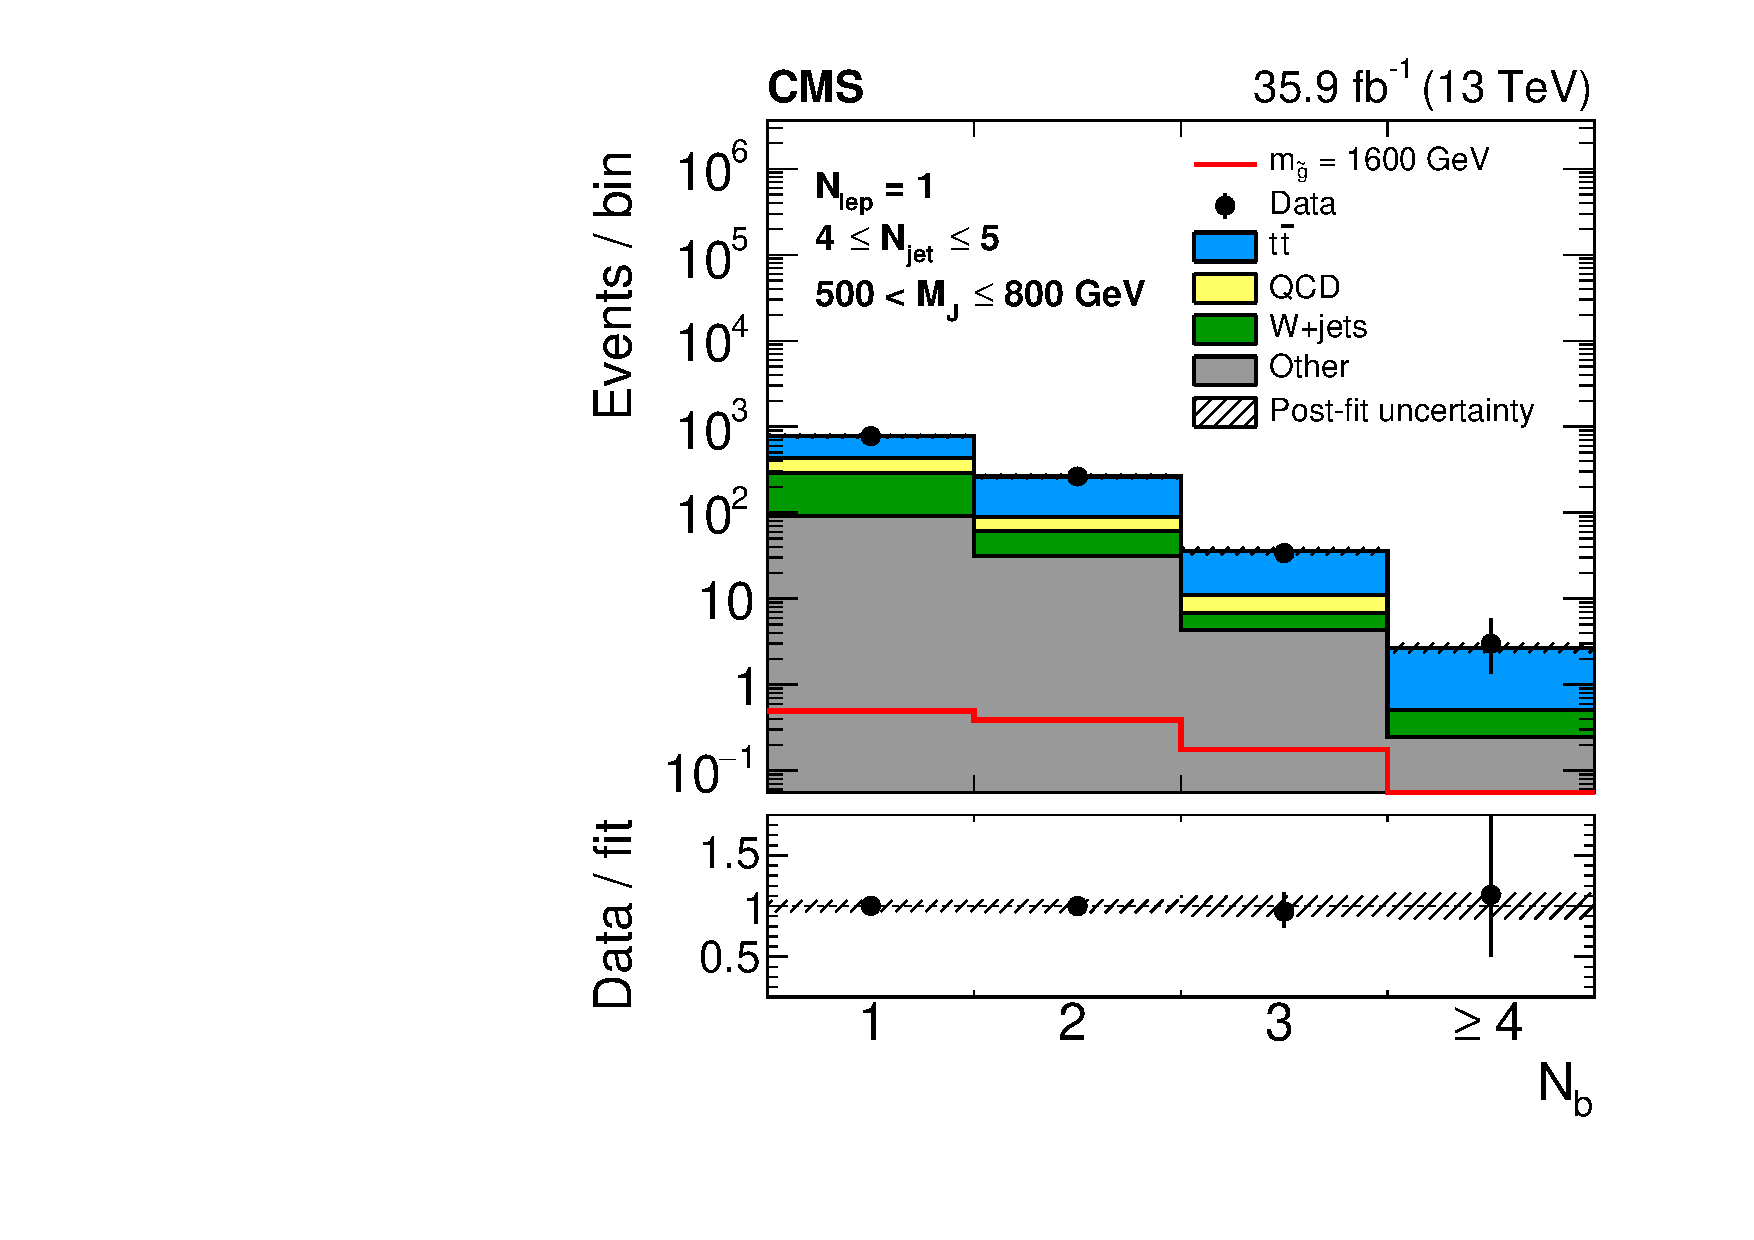
\includegraphics[angle=0,width=0.32\columnwidth]{fig/bonly_nlep1_nj45_lowmj.pdf}
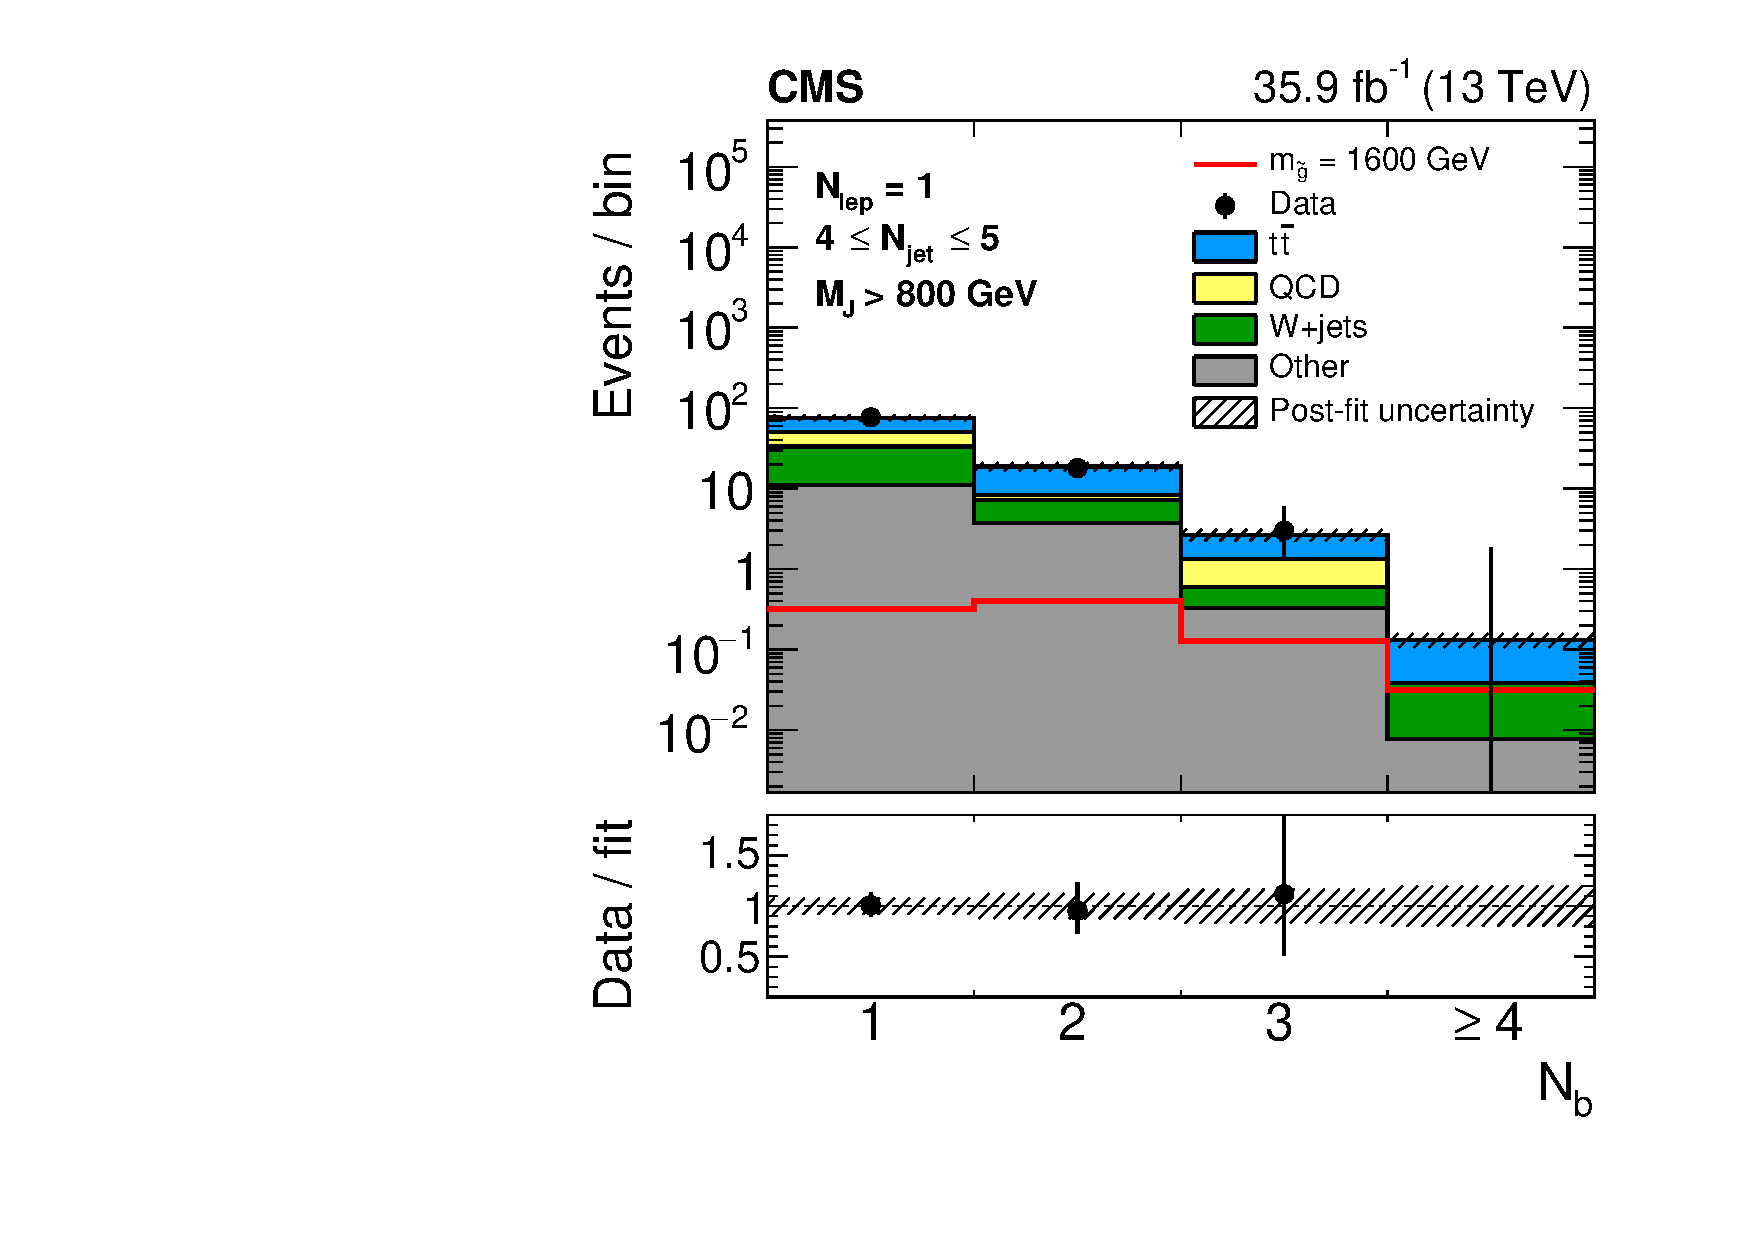
\includegraphics[angle=0,width=0.32\columnwidth]{fig/bonly_nlep1_nj45_highmj.pdf}
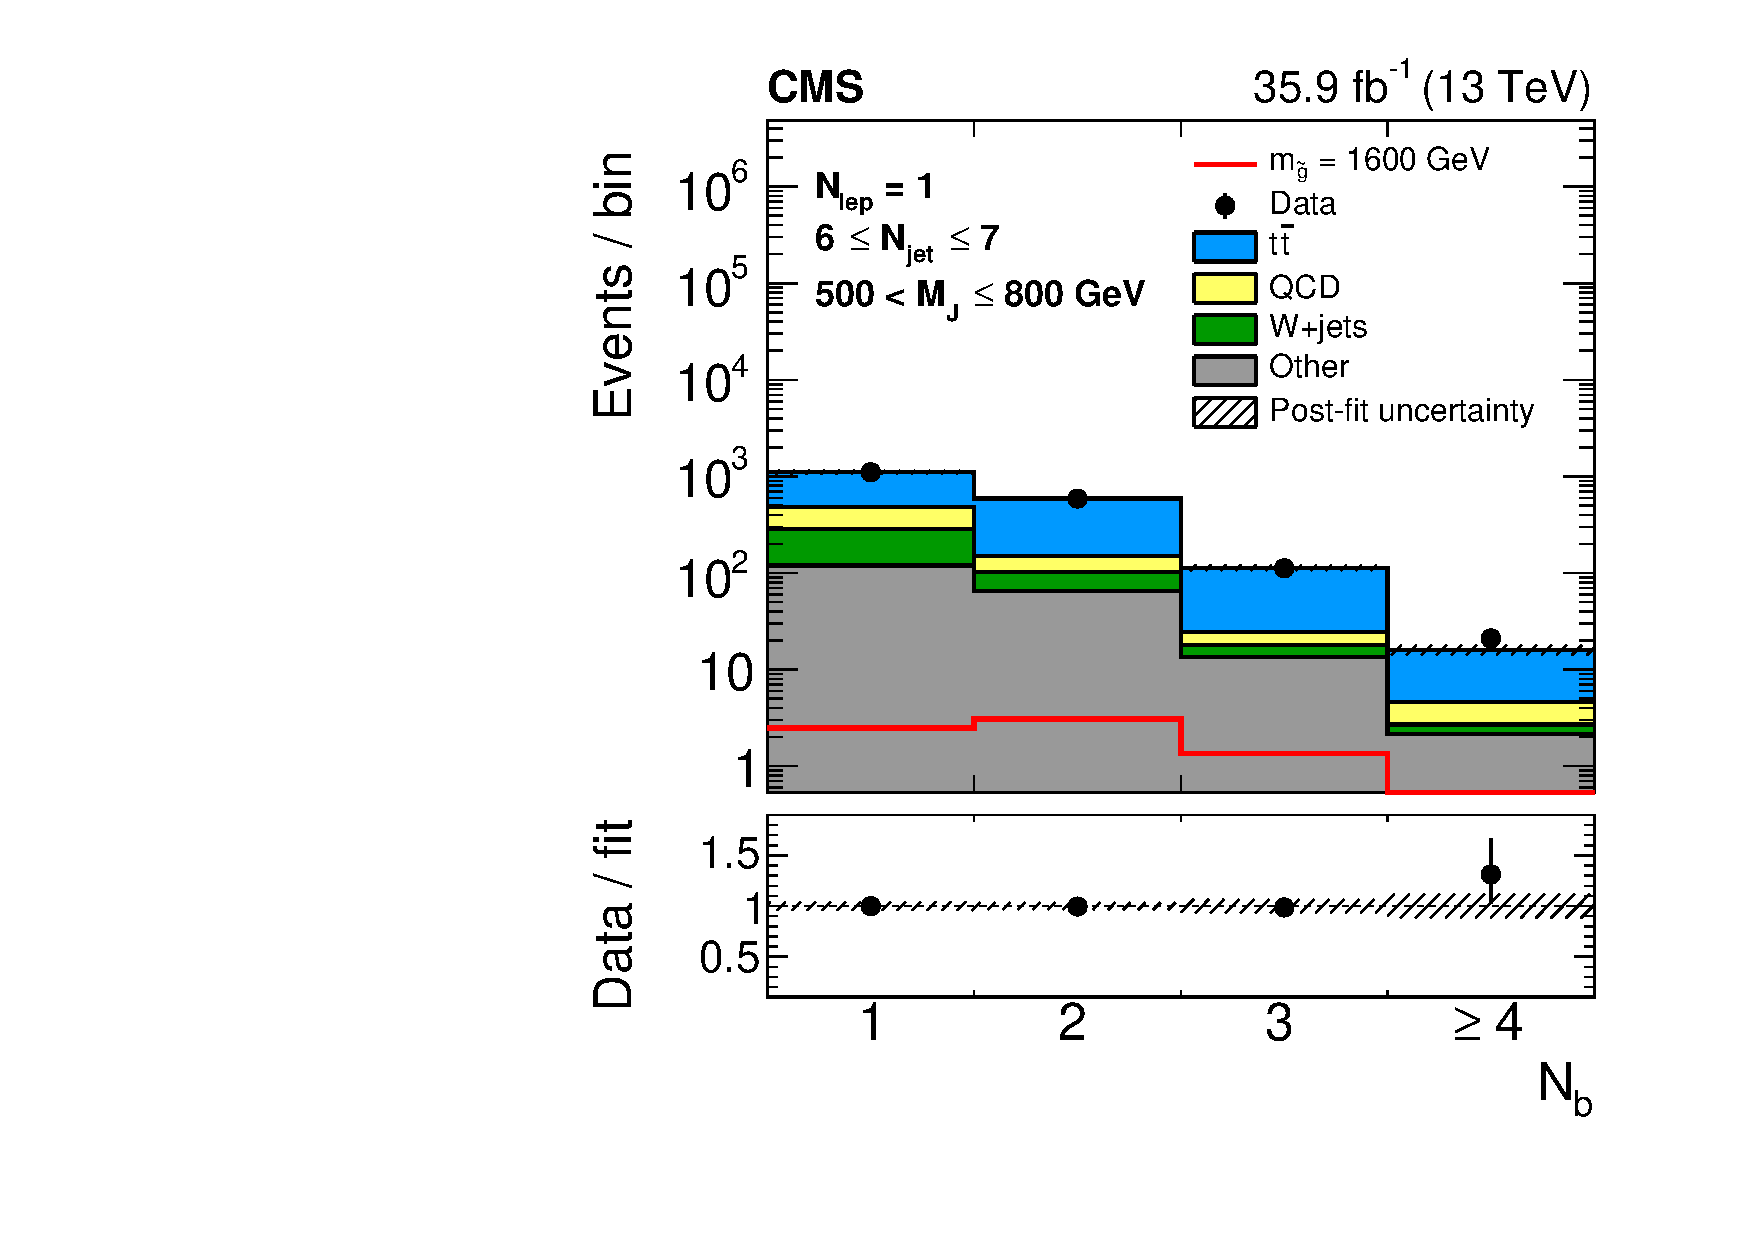
\includegraphics[angle=0,width=0.32\columnwidth]{fig/bonly_nlep1_nj67_lowmj.pdf}
\caption{Data and the background-only post-fit \Nb distribution for the control region bins: $4 \leq \Njets \leq 5$, $500 < \MJ \leq 800~\GeV$ (left), $4 \leq \Njets \leq 5$, $\MJ > 800~\GeV$ (middle), and $6 \leq \Njets \leq 7$, $500 < \MJ \leq 800~\GeV$ (right).
The expected signal distribution is also shown for a gluino mass of 1600~\GeV.
The ratio of data to post-fit yields is shown in the lower panel.
The post-fit uncertainty is depicted as a hatched band.}
\label{fig:bonly_cr}
\end{figure}

\begin{figure}[tbp!]
\centering
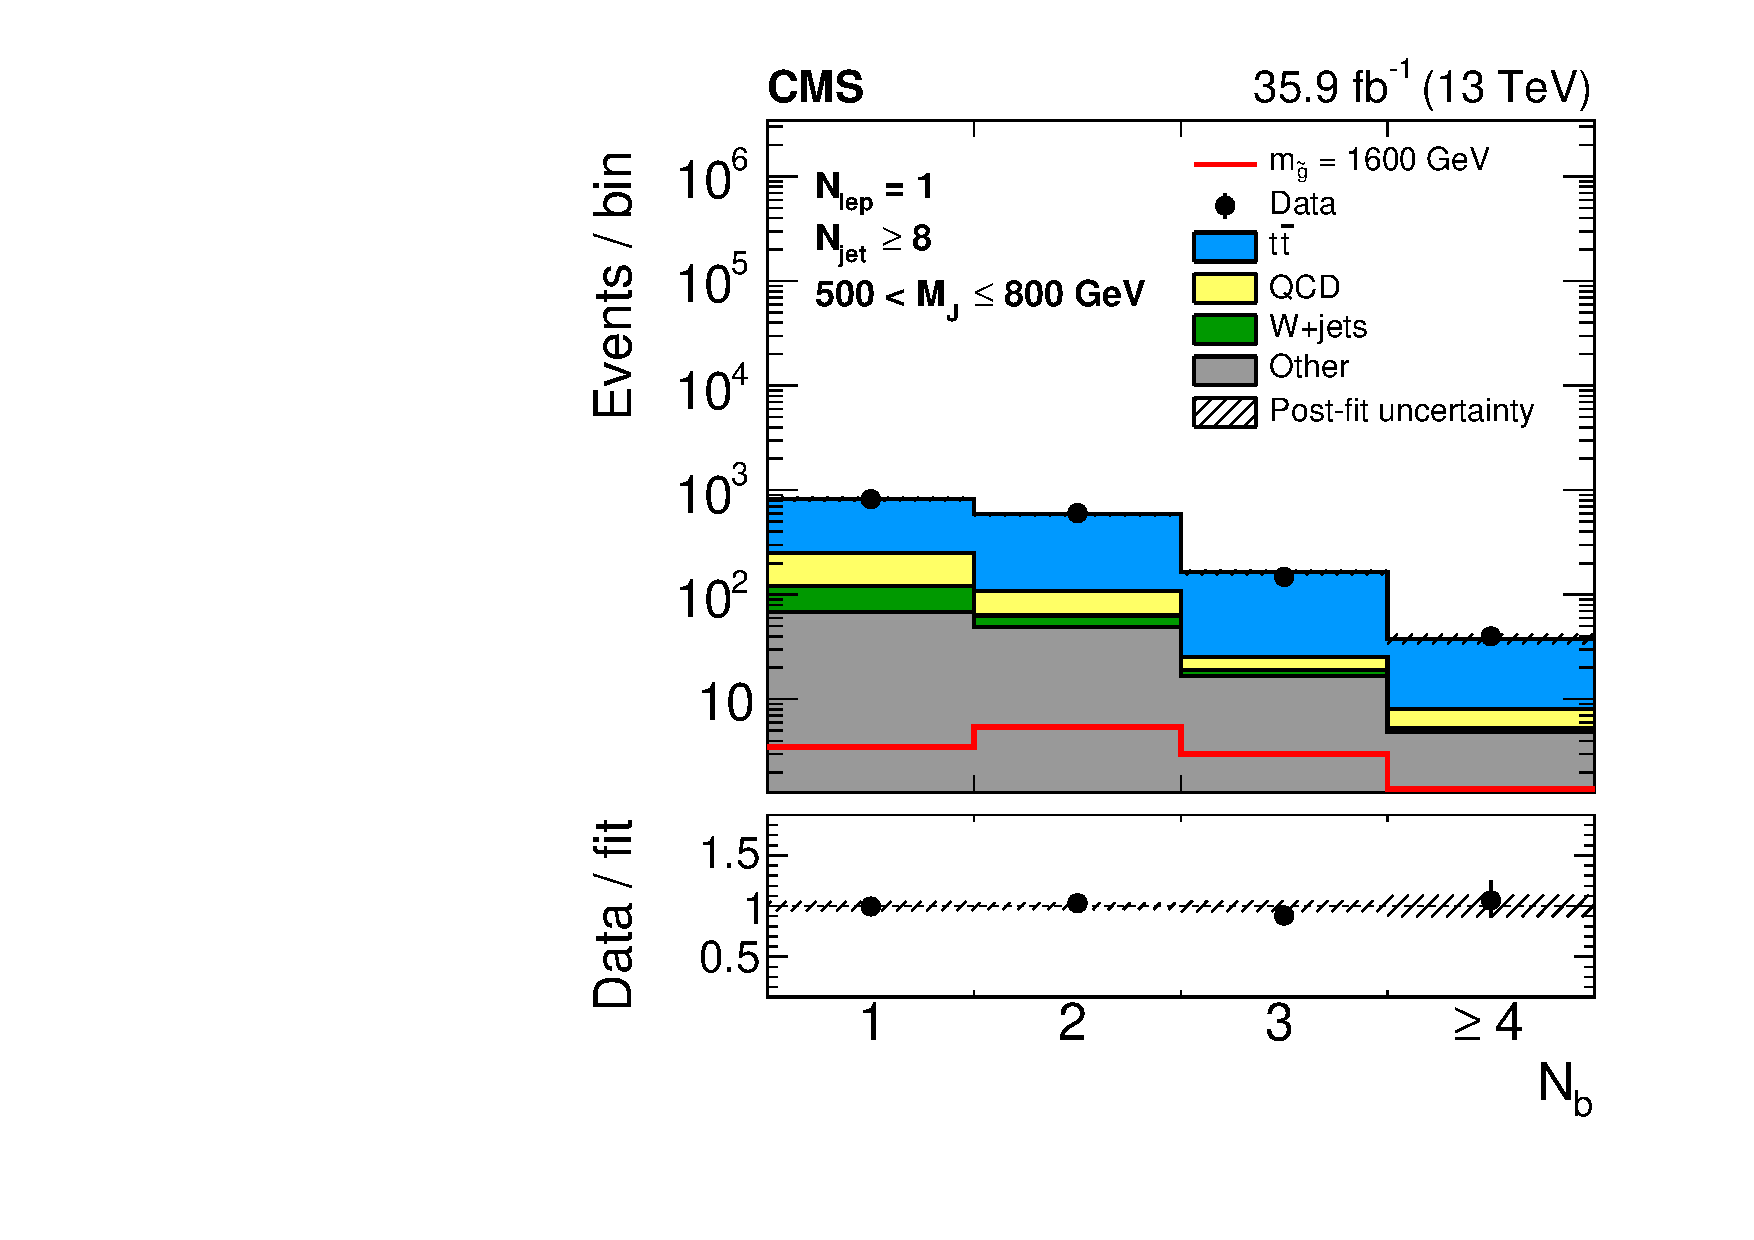
\includegraphics[angle=0,width=0.32\columnwidth]{fig/bonly_nlep1_nj8_lowmj.pdf}
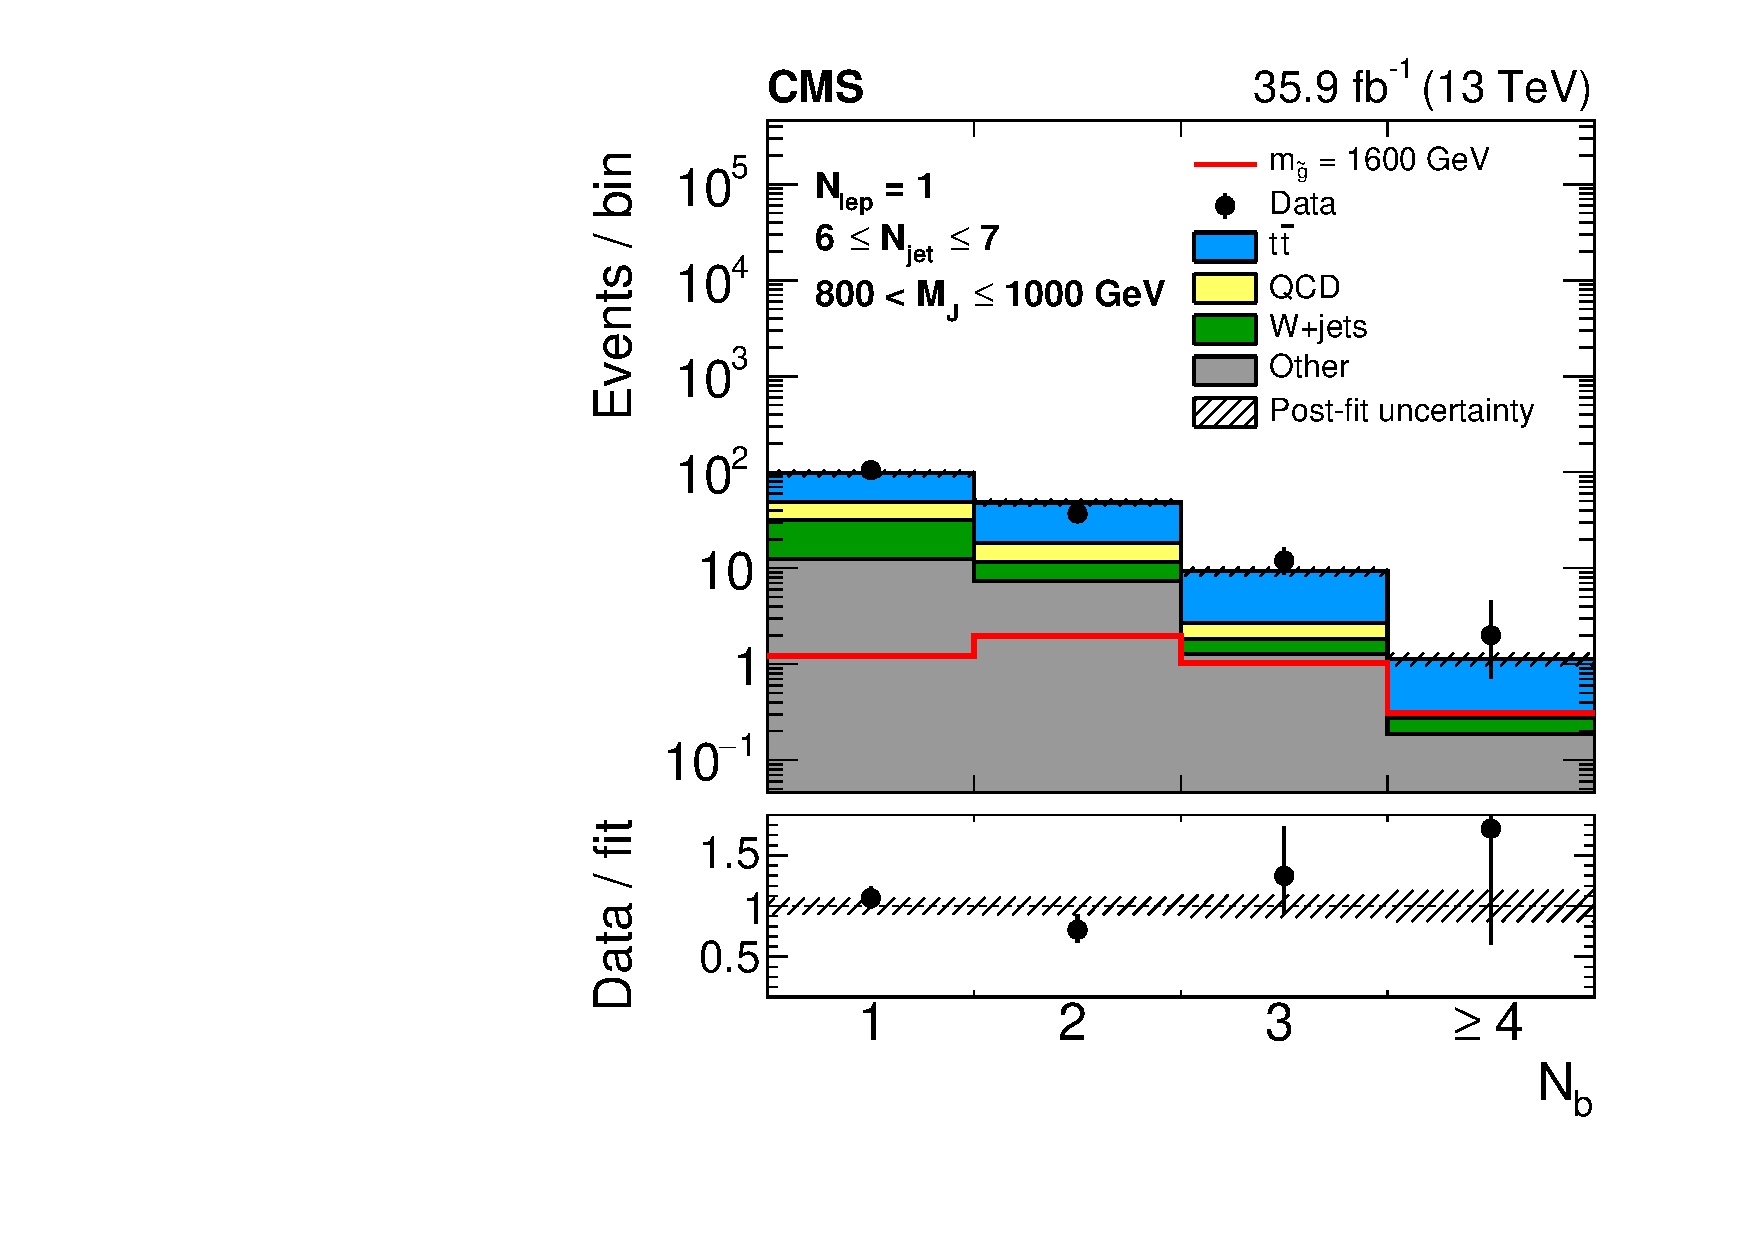
\includegraphics[angle=0,width=0.32\columnwidth]{fig/bonly_nlep1_nj67_highmj.pdf}
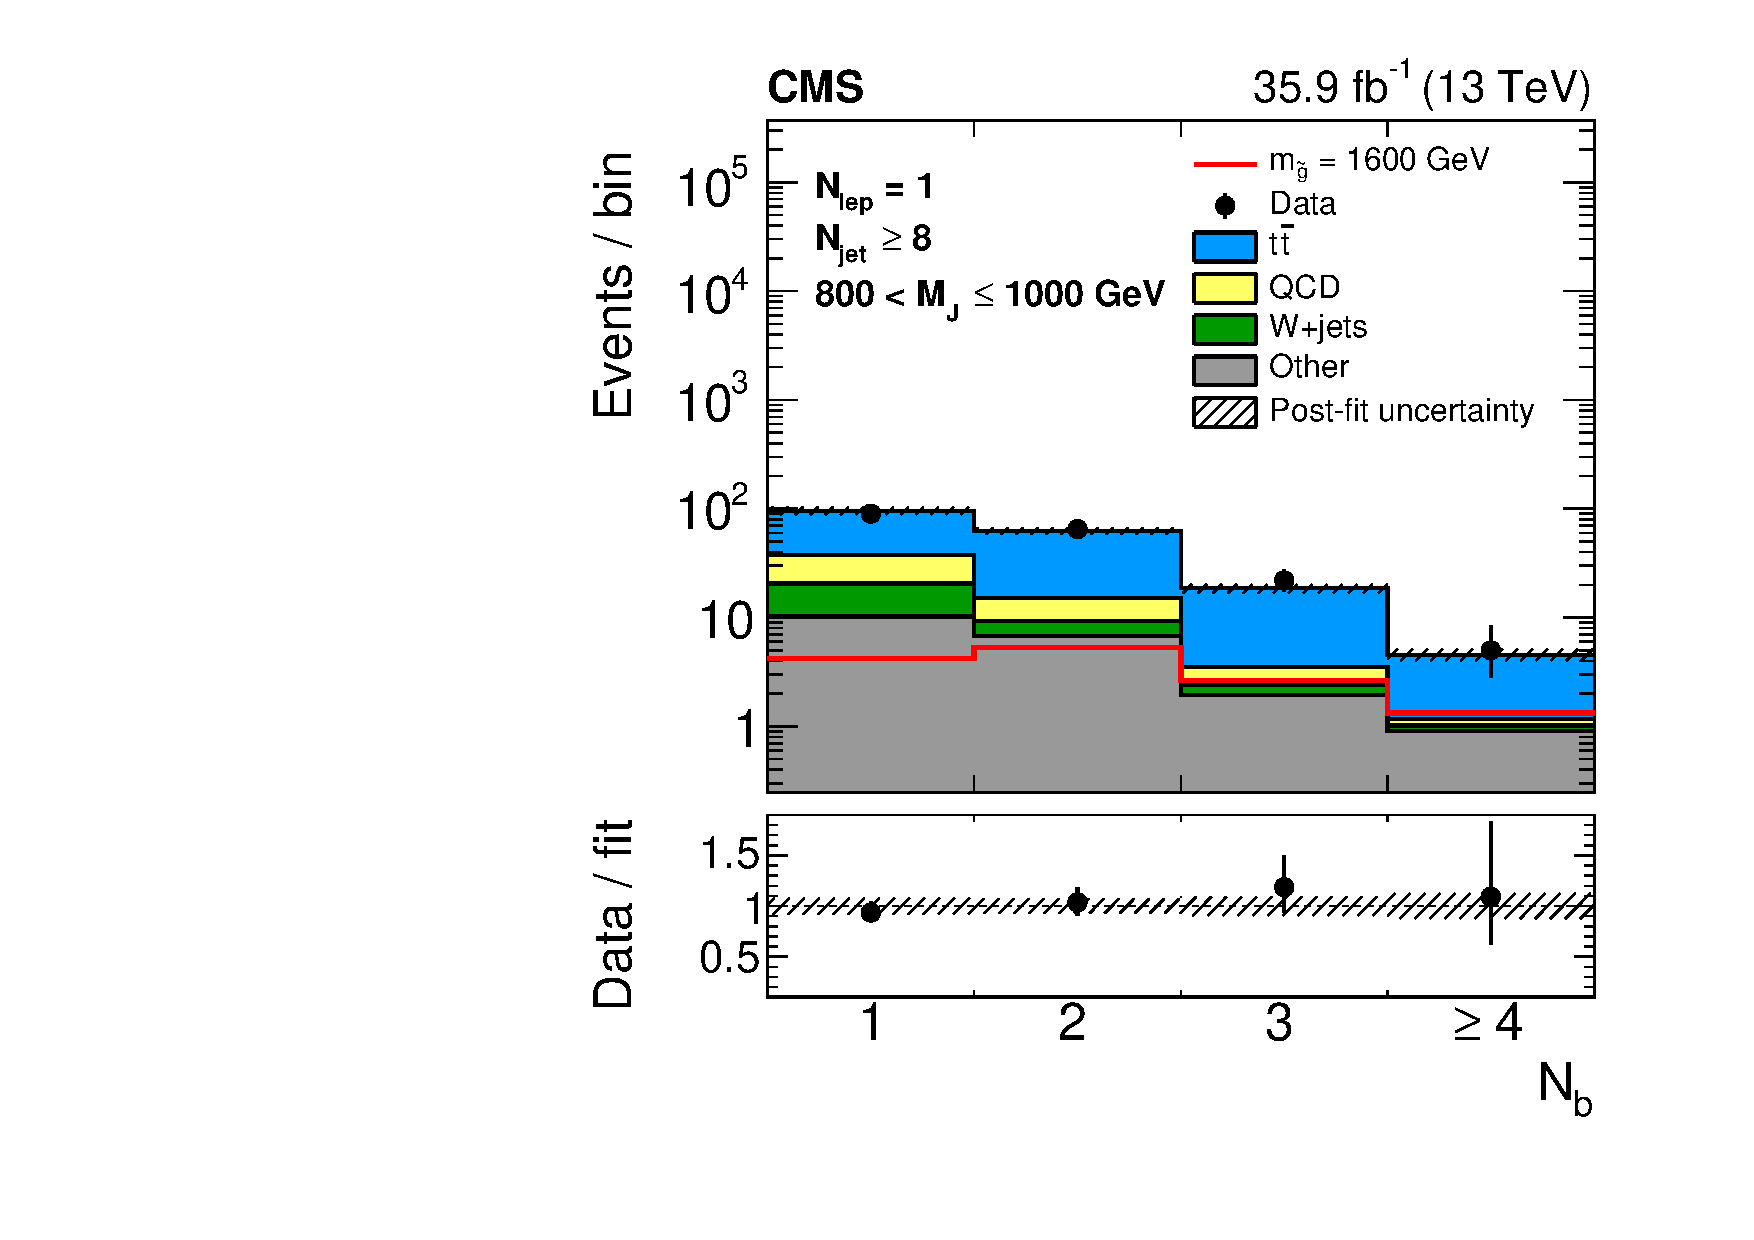
\includegraphics[angle=0,width=0.32\columnwidth]{fig/bonly_nlep1_nj8_highmj.pdf}
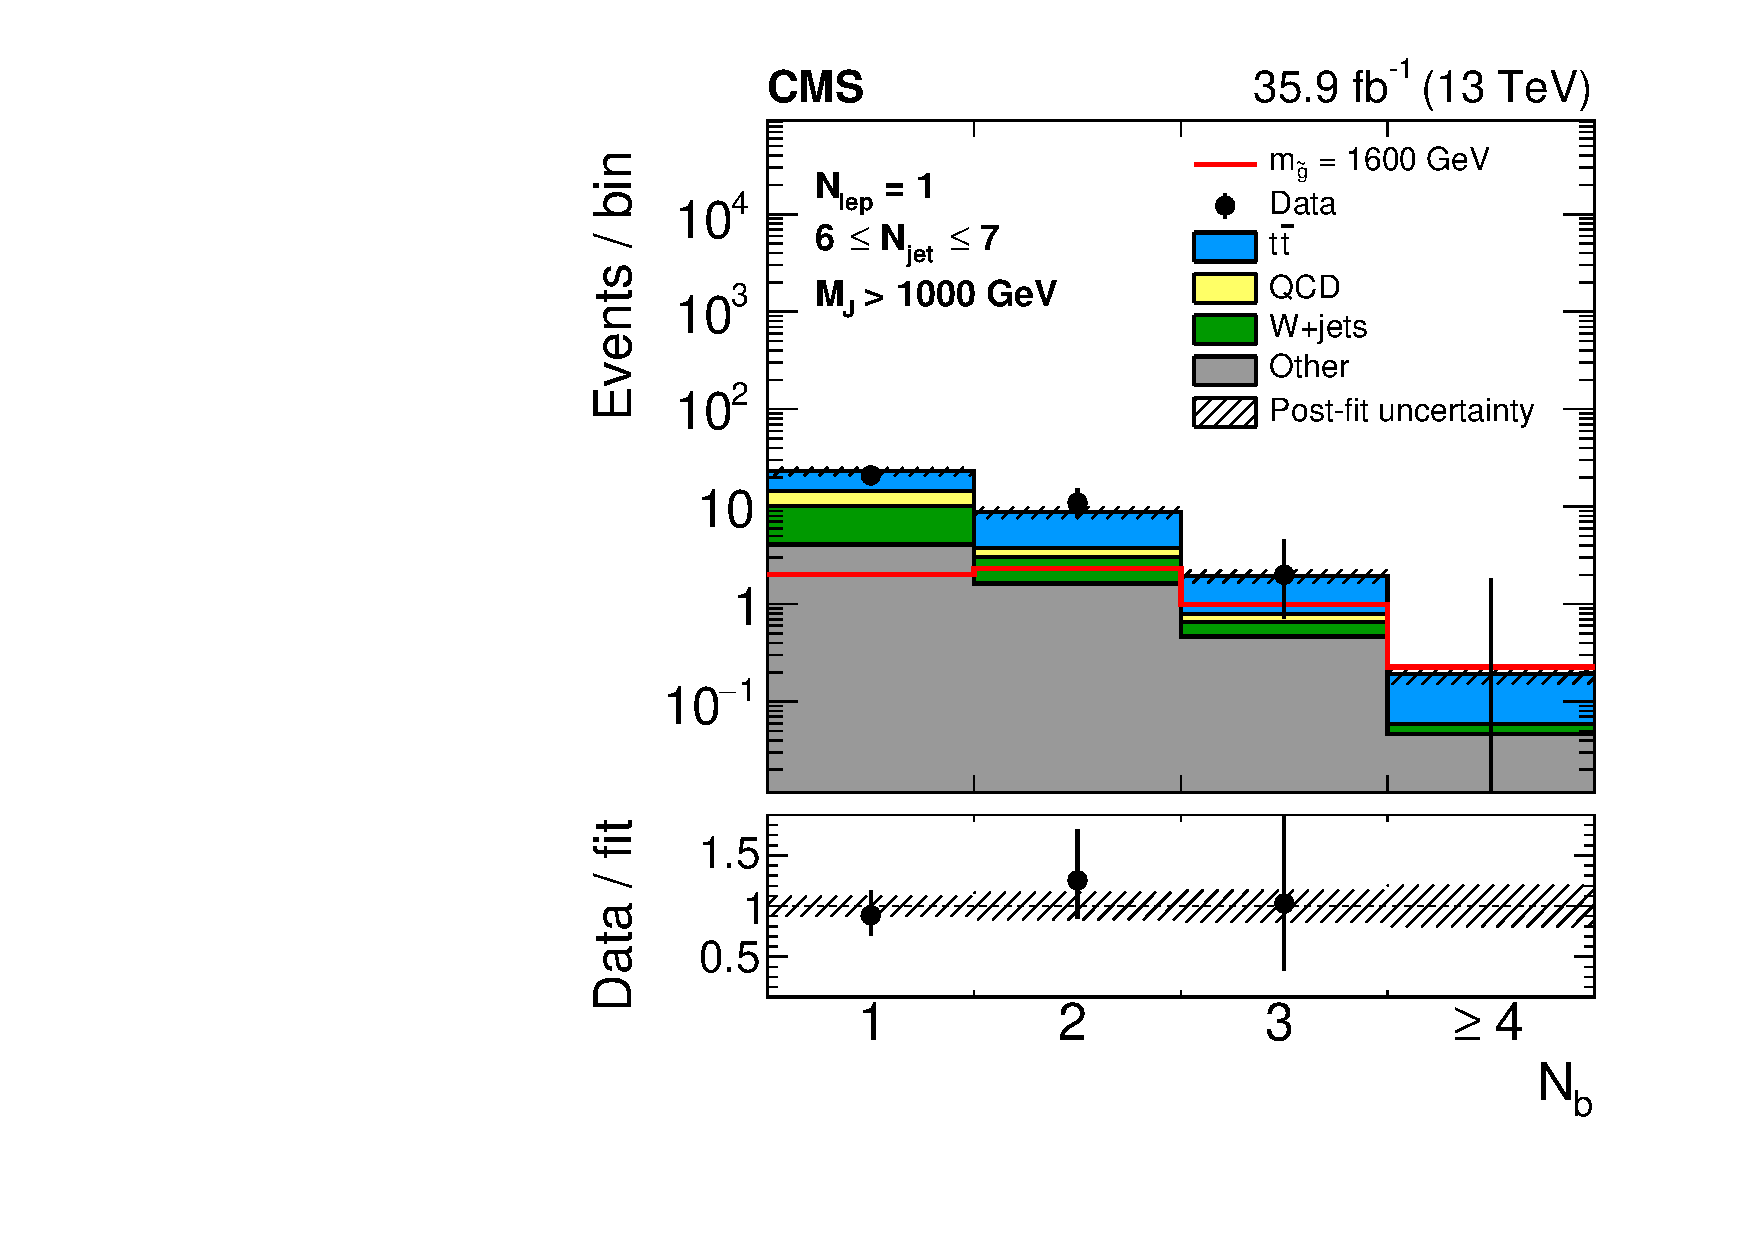
\includegraphics[angle=0,width=0.32\columnwidth]{fig/bonly_nlep1_nj67_vhighmj.pdf}
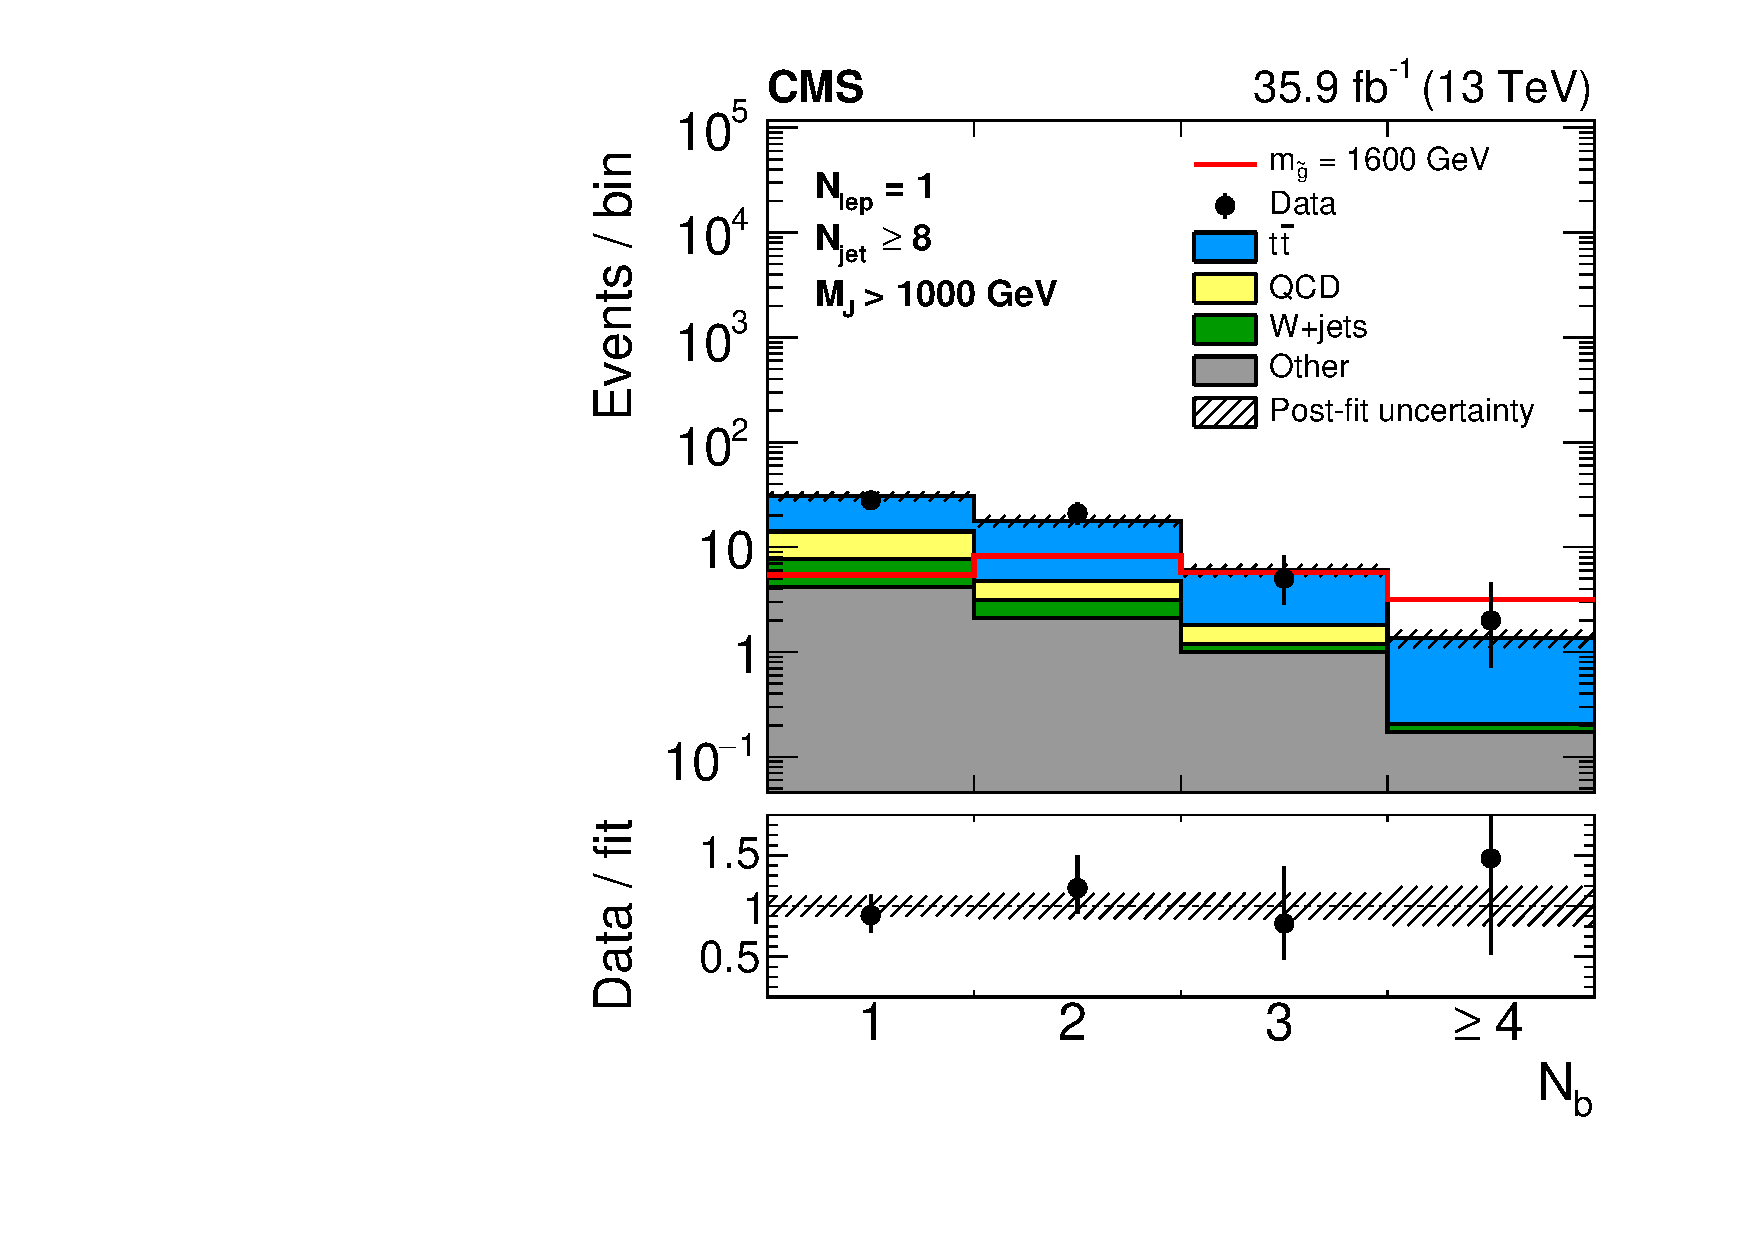
\includegraphics[angle=0,width=0.32\columnwidth]{fig/bonly_nlep1_nj8_vhighmj.pdf}
\caption{Data and the background-only post-fit \Nb distribution for the signal region bins: $\Njets \geq 8$, $500 < \MJ \leq 800~\GeV$ (upper-left), $6 \leq \Njets \leq 7$, $800 < \MJ \leq 1000~\GeV$ (upper-middle), $\Njets \geq 8$, $800 < \MJ \leq 1000~\GeV$ (upper-right), $ 6 \leq \Njets \leq 7$, $\MJ > 1000~\GeV$ (bottom-left), and $ \Njets \geq 8$, $\MJ > 1000~\GeV$ (bottom-right).
The expected signal distribution is also shown for a gluino mass of 1600~\GeV.
The ratio of data to post-fit yields is shown in the lower panel.
The post-fit uncertainty is depicted as a hatched band.}
\label{fig:bonly_sr}
\end{figure}

\begin{figure}[tbp!]
\centering
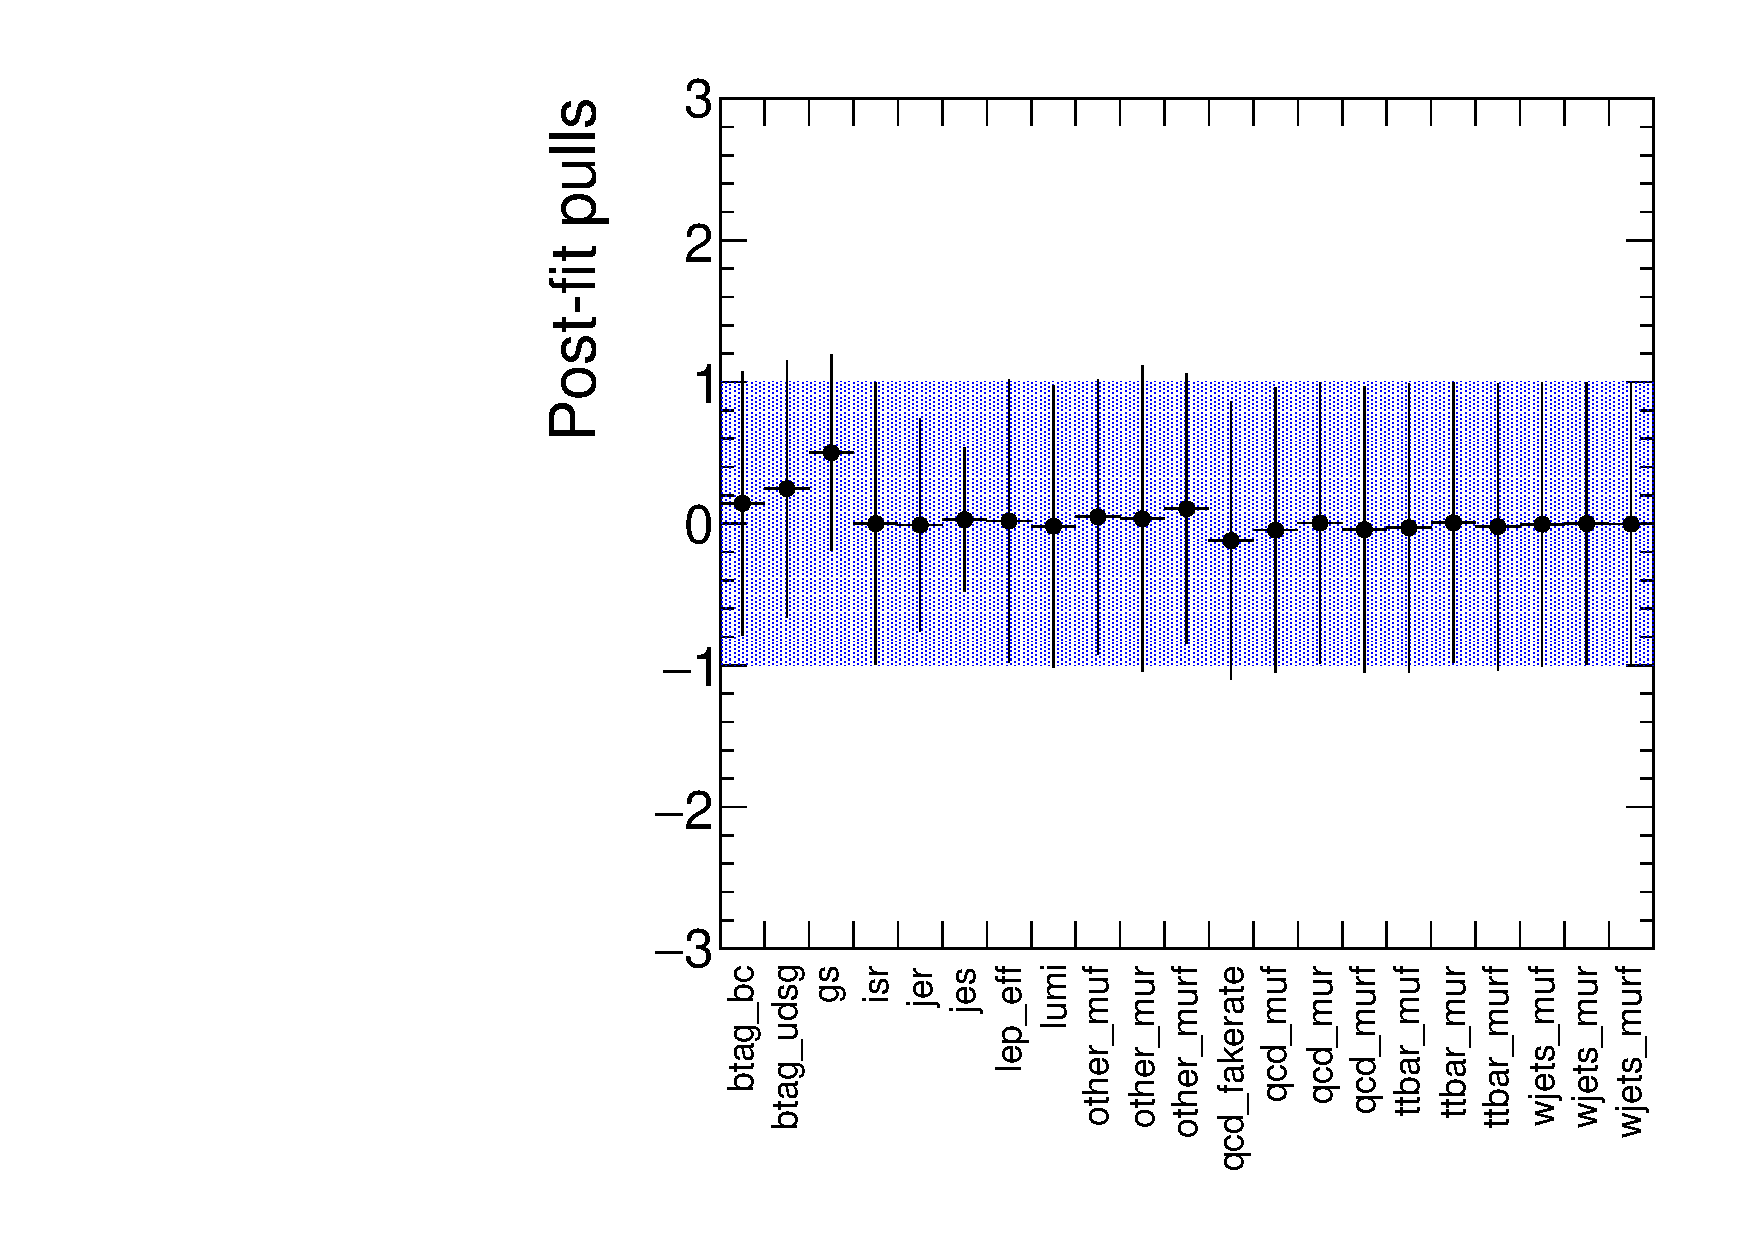
\includegraphics[angle=0,width=0.80\columnwidth]{fig/bonly_pulls.pdf}
\caption{Post-fit pulls of the background-only fit.
The post-fit value of the nuisance parameter is indicated by the data point, while the post-fit uncertainty is shown as a black line and is normalized by the pre-fit uncertainty depicted as the blue band.}
\label{fig:bonly_pulls}
\end{figure}

\begin{table}
\centering
\begin{tabular}[tbp!]{ l | c  c  c  c | c |  c | c  }
\hline
$\Nb$    & QCD    & \ttbar  & \Wjets & Other  & All bkg.      & Data   & Expected $\mglu = 1600~\GeV$ \\
\hline
\multicolumn{8}{c}{$4 \leq \Njets \leq 5$, $500 < \MJ \leq 800~\GeV$} \\
\hline
$1$       &  $148$   &  $340$    &  $196$  &  $91$    &  $775\pm43$     &  $777$  &  $0.50 \pm 0.13$ \\
$2$       &  $29$    &  $175$    &  $30$   &  $31$    &  $264\pm17$     &  $264$  &  $0.39 \pm 0.11$ \\
$3$       &  $4.3$   &  $24.8$   &  $2.5$  &  $4.4$   &  $36\pm4$       &  $34$   &  $0.18 \pm 0.08$ \\
$\geq 4$  &  $0.0$   &  $2.2$    &  $0.3$  &  $0.2$   &  $2.7\pm0.4$    &  $3$    &  $0.04 \pm 0.04$ \\
\hline
\multicolumn{8}{c}{$4 \leq \Njets \leq 5$, $\MJ > 800~\GeV$} \\
\hline
$1$       &  $16.5$  &  $26.3$   &  $22.5$ &  $11.0$  &  $76\pm6$       &  $77$    &  $0.32 \pm 0.11$ \\
$2$       &  $1.1$   &  $10.6$   &  $3.4$  &  $3.8$   &  $19\pm2$       &  $18$    &  $0.40 \pm 0.12$ \\
$3$       &  $0.7$   &  $1.3$    &  $0.3$  &  $0.3$   &  $2.7\pm0.5$    &  $3$     &  $0.13 \pm 0.06$ \\
$\geq 4$  &  $0.00$  &  $0.09$   &  $0.03$ &  $0.01$  &  $0.13\pm0.03$  &  $0$     &  $0.03 \pm 0.03$ \\
\hline
\multicolumn{8}{c}{$6 \leq \Njets \leq 7$, $500 < \MJ \leq 800~\GeV$} \\
\hline
$1$       &  $197$   &  $620$    &  $169$  &  $120$   &  $1106\pm48$    &  $1105$  &  $2.5 \pm 0.3$   \\
$2$       &  $49$    &  $440$    &  $36$   &  $66$    &  $591\pm21$     &  $588$   &  $3.1 \pm 0.3$   \\
$3$       &  $6.4$   &  $89.2$   &  $4.6$  &  $13.4$  &  $114\pm8$      &  $112$   &  $1.4 \pm 0.2$   \\
$\geq 4$  &  $1.9$   &  $11.4$   &  $0.6$  &  $2.1$   &  $16\pm2$       &  $21$    &  $0.25 \pm 0.09$ \\
\hline
\multicolumn{8}{c}{$\Njets \geq 8$, $500 < \MJ \leq 800~\GeV$} \\
\hline
$1$       &  $130$   &  $574$   &  $53$    &  $68$    &  $825\pm38$     &  $821$   &  $3.5 \pm 0.3$   \\
$2$       &  $45$    &  $478$   &  $14$    &  $49$    &  $586\pm20$     &  $603$   &  $5.4 \pm 0.4$   \\
$3$       &  $6.3$   &  $138.1$ &  $2.5$   &  $16.7$  &  $164\pm9$      &  $148$   &  $3.0 \pm 0.3$   \\
$\geq 4$  &  $2.8$   &  $29.8$  &  $0.4$   &  $4.8$   &  $38\pm4$       &  $40$    &  $1.4 \pm 0.2$   \\
\hline
\multicolumn{8}{c}{$6 \leq \Njets \leq 7$, $800 < \MJ \leq 1000~\GeV$} \\
\hline
$1$       &  $17.3$  &  $48.4$  &  $19.2$  &  $12.3$  &  $97\pm8$       &  $105$   &  $1.2 \pm 0.2$   \\
$2$       &  $6.6$   &  $30.1$  &  $4.3$   &  $7.3$   &  $48\pm4$       &  $37$    &  $2.0 \pm 0.3$   \\
$3$       &  $0.8$   &  $6.6$   &  $0.5$   &  $1.3$   &  $9.3\pm1.0$    &  $12$    &  $1.0 \pm 0.2$   \\
$\geq 4$  &  $0.0$   &  $0.9$   &  $0.1$   &  $0.2$   &  $1.1\pm0.2$    &  $2$     &  $0.31 \pm 0.09$ \\
\hline
\multicolumn{8}{c}{$\Njets \geq 8$, $800 < \MJ \leq 1000~\GeV$} \\
\hline
$1$       &  $17.0$  &  $58.7$  &  $10.3$  &  $10.2$  &  $96\pm8$       &  $90$    &  $4.2 \pm 0.4$   \\
$2$       &  $5.8$   &  $47.5$  &  $2.5$   &  $6.8$   &  $63\pm5$       &  $65$    &  $5.3 \pm 0.4$   \\
$3$       &  $1.1$   &  $15.0$  &  $0.4$   &  $2.0$   &  $19\pm2$       &  $22$    &  $2.6 \pm 0.3$   \\
$\geq 4$  &  $0.2$   &  $3.4$   &  $0.1$   &  $0.9$   &  $4.6\pm0.6$    &  $5$     &  $1.3 \pm 0.2$   \\
\hline
\multicolumn{8}{c}{$6 \leq \Njets \leq 7$, $\MJ > 1000~\GeV$} \\
\hline
$1$       &  $4.4$   &  $8.7$   &  $6.0$  &  $4.1$  &  $23\pm2$         &  $21$    &  $2.0 \pm 0.3$   \\
$2$       &  $0.7$   &  $5.0$   &  $1.4$  &  $1.6$  &  $8.8\pm1.2$      &  $11$    &  $2.3 \pm 0.3$   \\
$3$       &  $0.1$   &  $1.2$   &  $0.2$  &  $0.5$  &  $1.9\pm0.3$      &  $2$     &  $1.0 \pm 0.2$   \\
$\geq 4$  &  $0.00$  &  $0.13$  &  $0.01$ &  $0.05$ &  $0.19\pm0.04$    &  $0$     &  $0.23 \pm 0.08$ \\
\hline
\multicolumn{8}{c}{$\Njets \geq 8$, $\MJ > 1000~\GeV$} \\
\hline
$1$       &  $6.4$   &  $16.7$  &  $3.5$  &  $4.1$  &  $31\pm3$         &  $28$    &  $5.4 \pm 0.4$   \\
$2$       &  $1.6$   &  $13.1$  &  $1.1$  &  $2.1$  &  $18\pm2$         &  $21$    &  $8.2 \pm 0.5$   \\
$3$       &  $0.6$   &  $4.2$   &  $0.2$  &  $1.0$  &  $6.0\pm0.8$      &  $5$     &  $5.7 \pm 0.4$   \\
$\geq 4$  &  $0.0$   &  $1.2$   &  $0.0$  &  $0.2$  &  $1.4\pm0.3$      &  $2$     &  $3.2 \pm 0.3$   \\
\hline
\end{tabular}
\caption{Post-fit yields of the background-only fit, observed data, and expected yields for $\mglu = 1600~\GeV$.}
\label{tab:bonly_yields}
\end{table}

The good description of the observed data as well as the behavior of the nuisance parmeters match the pre-fit expectations outlined in Section~\ref{sec:prefit_data}.
An additional indication that the background-only fit is well-behaved is that the post-fit nuisance parameter values are in good agreement with those of the control-region fit.
This suggests that the measurements of the nuisance parameters in the background-dominated control regions are able to largely describe the difference in \Nb shape between simulation and data in the signal regions without the need of a signal contribution.

\end{subsection}

\begin{subsection}{Signal-plus-background Fit Results}

A signal-plus-background fit is performed for gluino masses ranging from 1000 to 2000~\GeV.
For all masses, the post-fit \Nb distribution describes the data well, and the fit extracts at most a small and insignificant signal contribution.

For example, the fitted signal strength for a model corresponding to a $1600~\GeV$ gluno is $\mu = 0.18^{+0.41}_{-0.18}$ with the post-fit \Nb distributions shown in Figure~\ref{fig:splusb_cr} and Figure~\ref{fig:splusb_sr} for the control and signal region bins, respectively.
The post-fit values of the nuisance parameters are small and consistent with those of the background-only fit, as shown in Table~\ref{tab:fit_pulls}.

Given the post-fit agreement of the \Nb distributions, well-behaved nuisance parameters, and insignificant fitted signal strength, no evidence for a signal corresponding to the T1tbs model is observed.

\begin{figure}[tbp!]
\centering
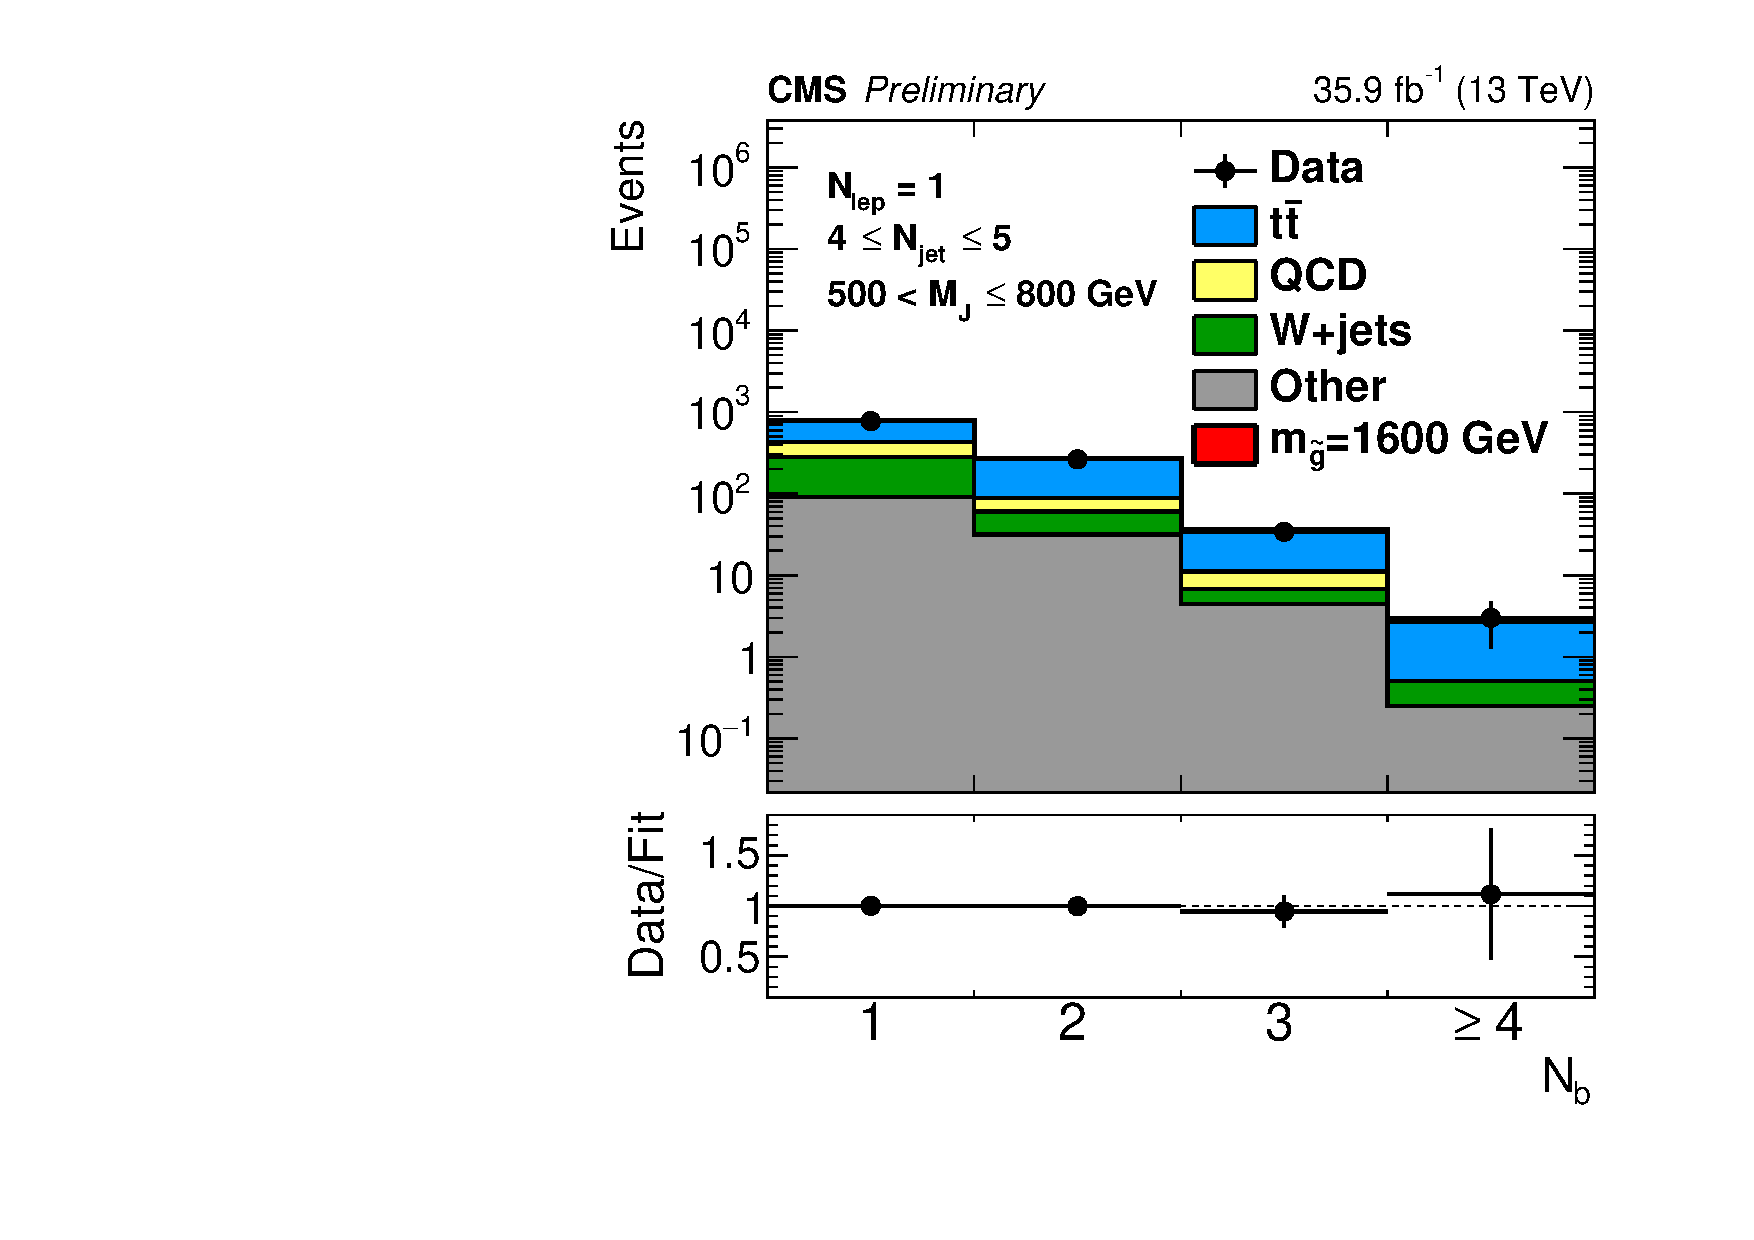
\includegraphics[angle=0,width=0.32\columnwidth]{fig/splusb_nlep1_nj45_lowmj.pdf}
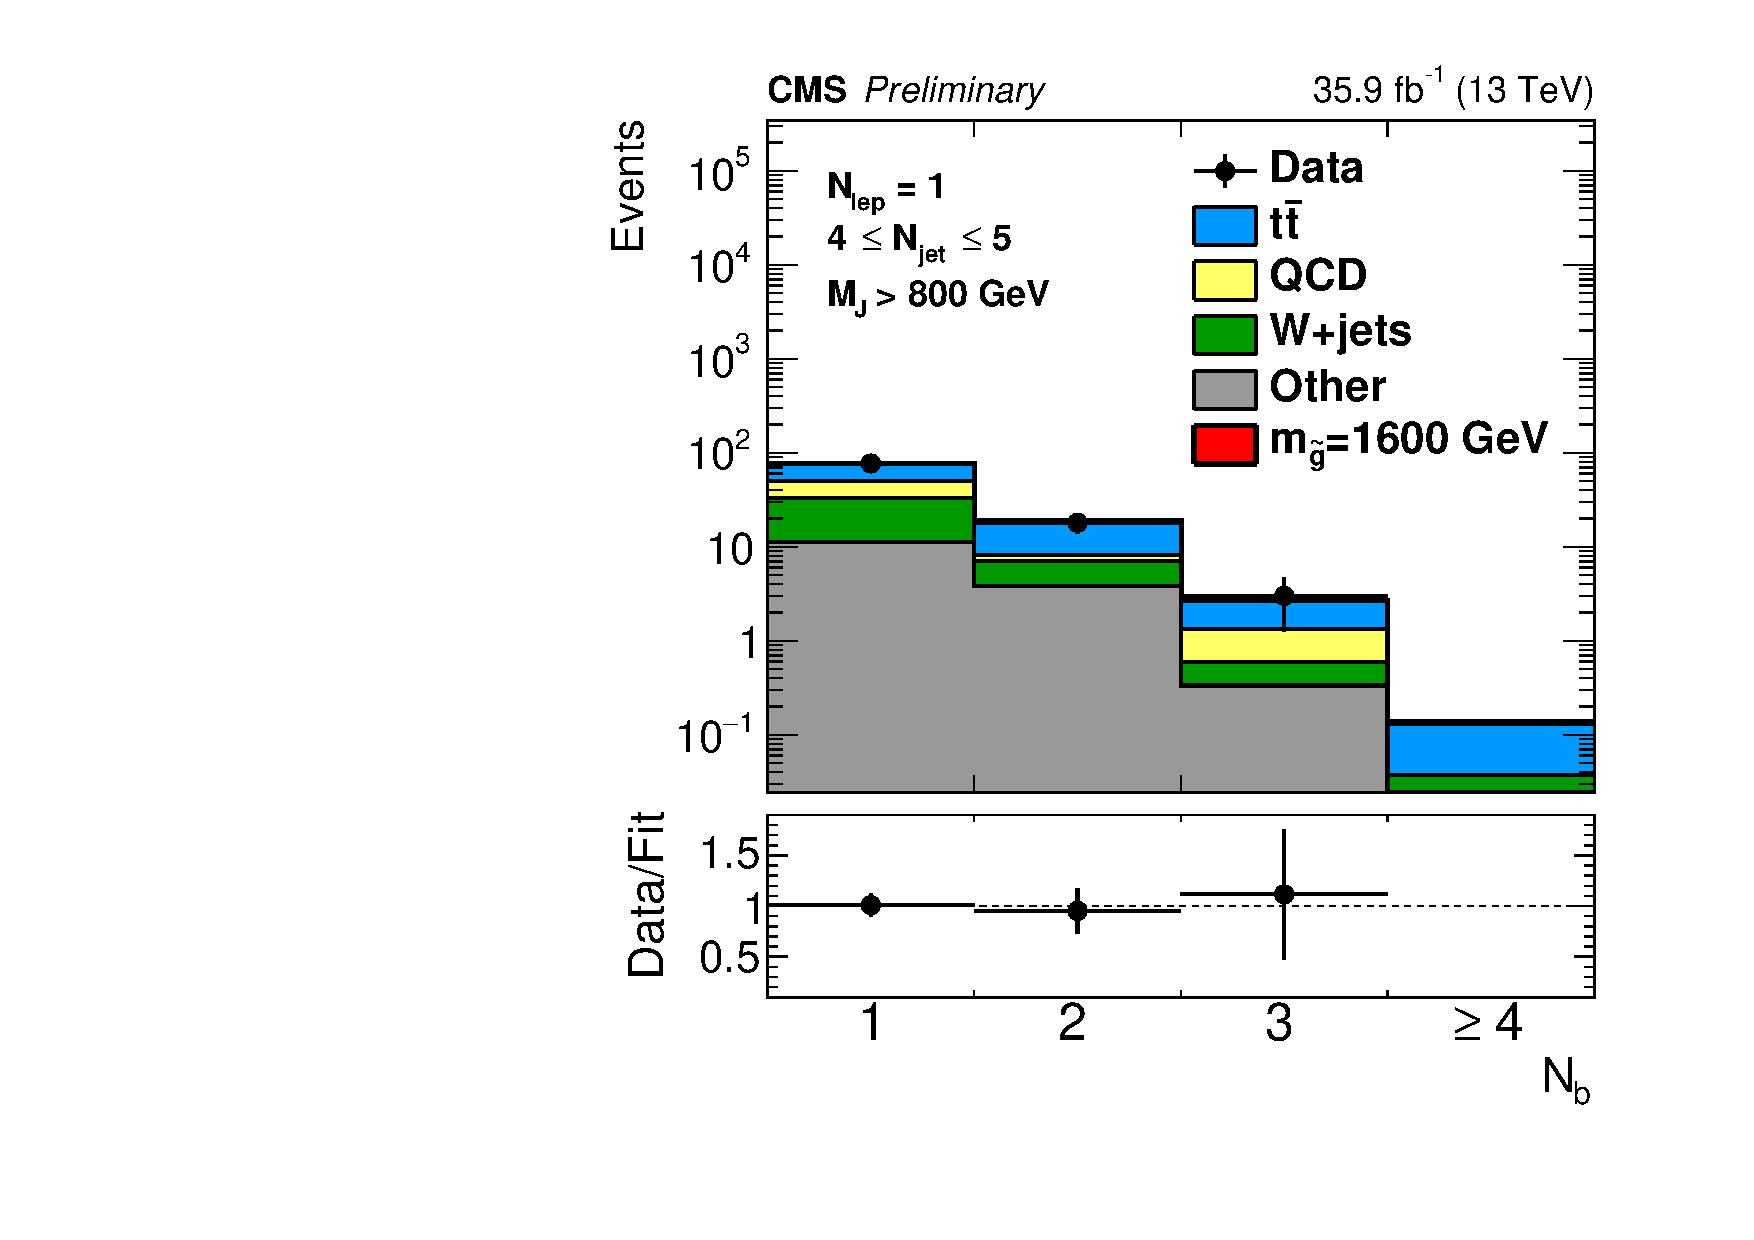
\includegraphics[angle=0,width=0.32\columnwidth]{fig/splusb_nlep1_nj45_highmj.pdf}
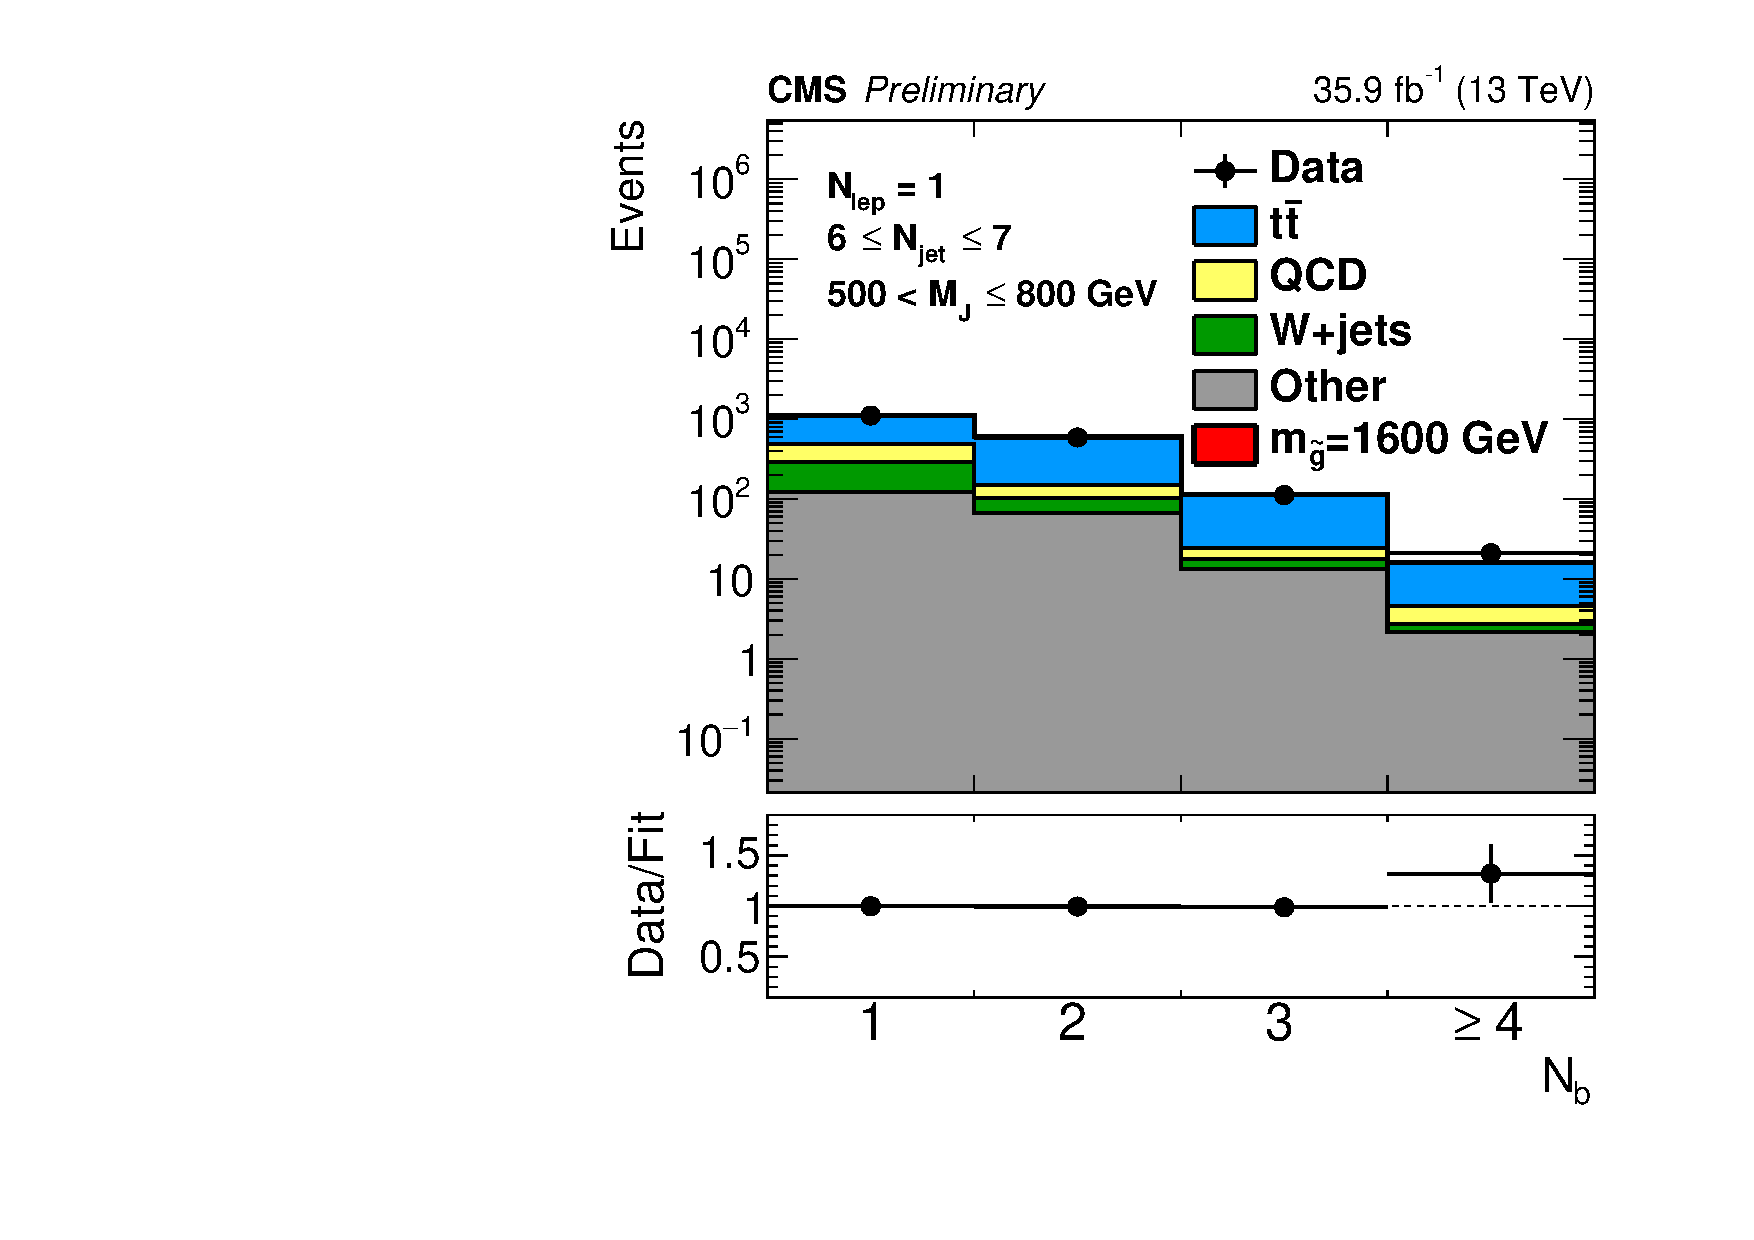
\includegraphics[angle=0,width=0.32\columnwidth]{fig/splusb_nlep1_nj67_lowmj.pdf}
\caption{Data and the $\mglu = 1600~\GeV$ signal-plus-background post-fit \Nb distribution for the control region bins: $4 \leq \Njets \leq 5$, $500 < \MJ \leq 800~\GeV$ (left), $4 \leq \Njets \leq 5$, $\MJ > 800~\GeV$ (right), and $6 \leq \Njets \leq 7$, $500 < \MJ \leq 800~\GeV$ (middle).
The ratio of data to post-fit yields is shown in the lower panel.
The post-fit uncertainty is depicted as a hatched band.}
\label{fig:splusb_cr}
\end{figure}

\begin{figure}[tbp!]
\centering
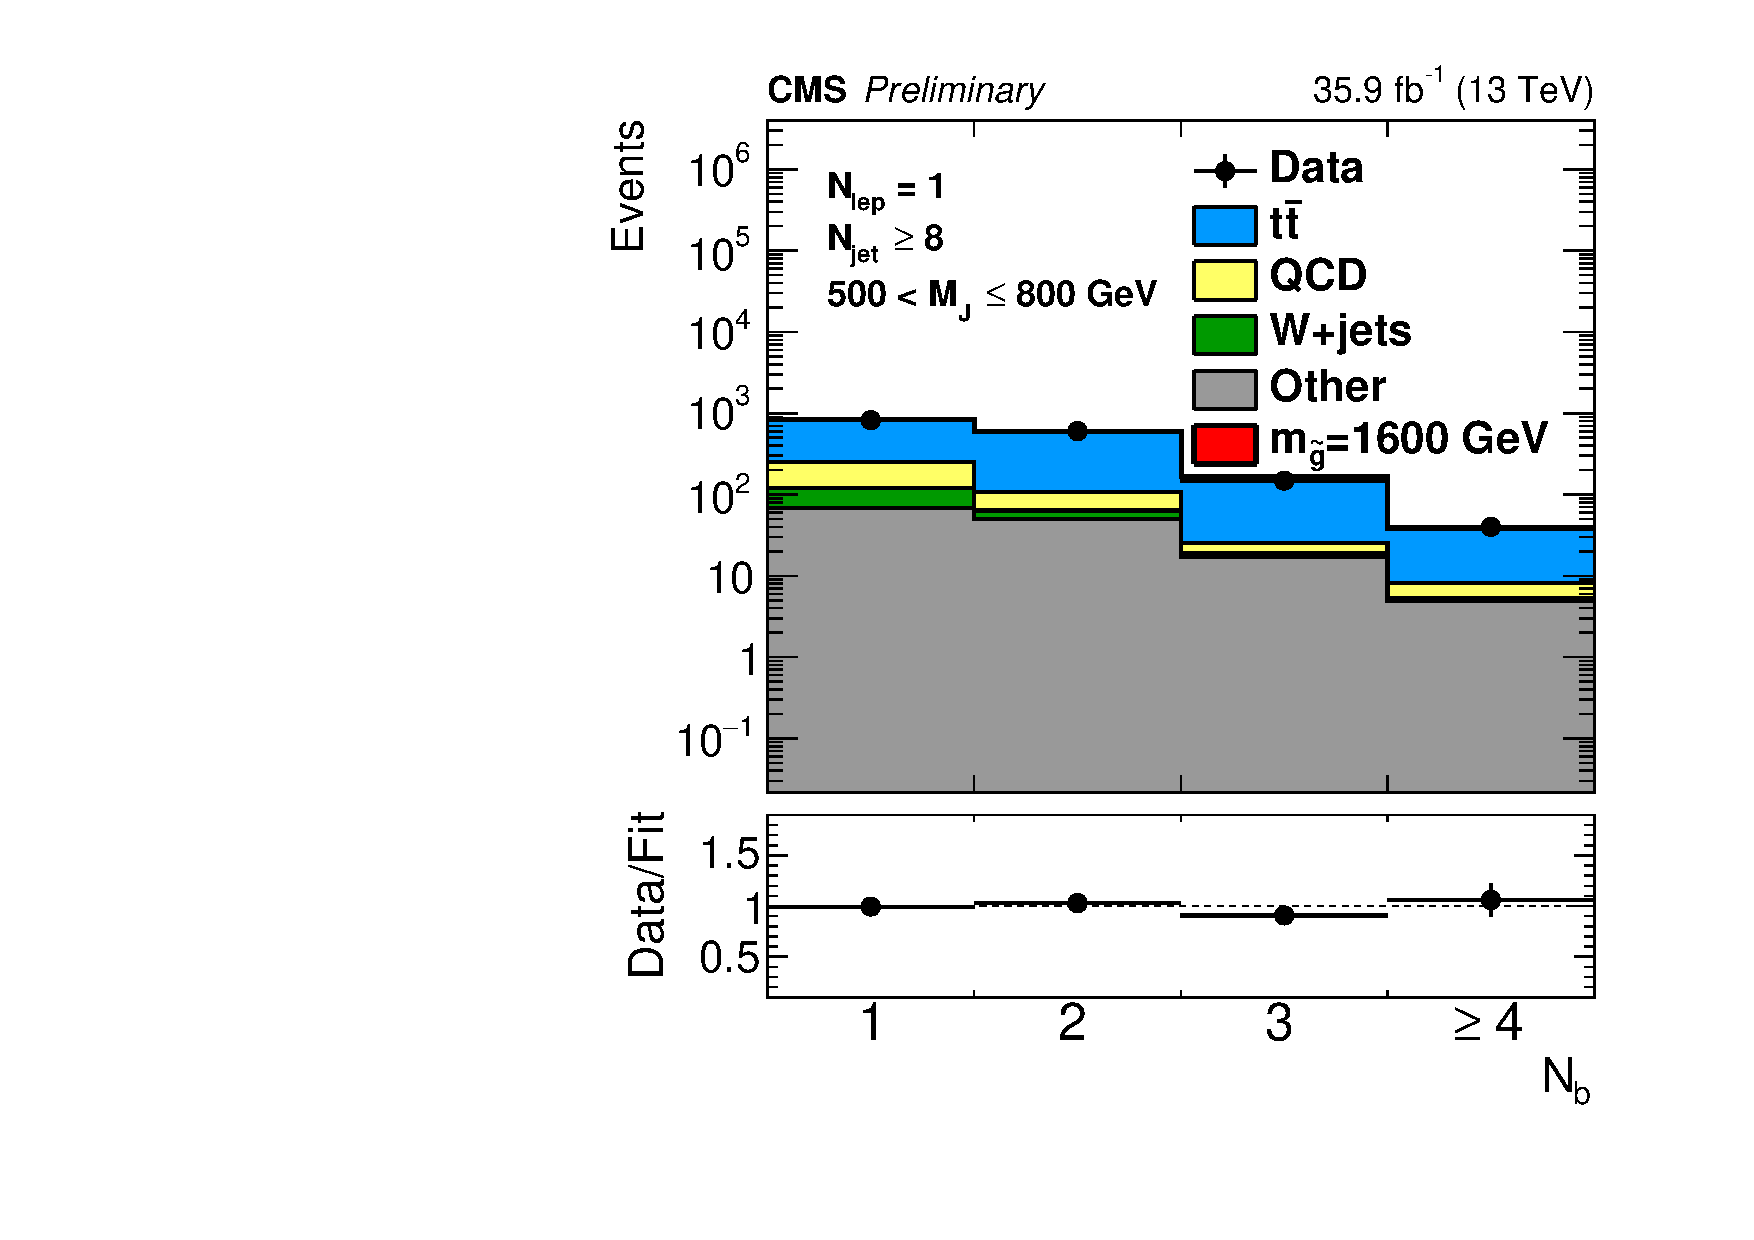
\includegraphics[angle=0,width=0.32\columnwidth]{fig/splusb_nlep1_nj8_lowmj.pdf}
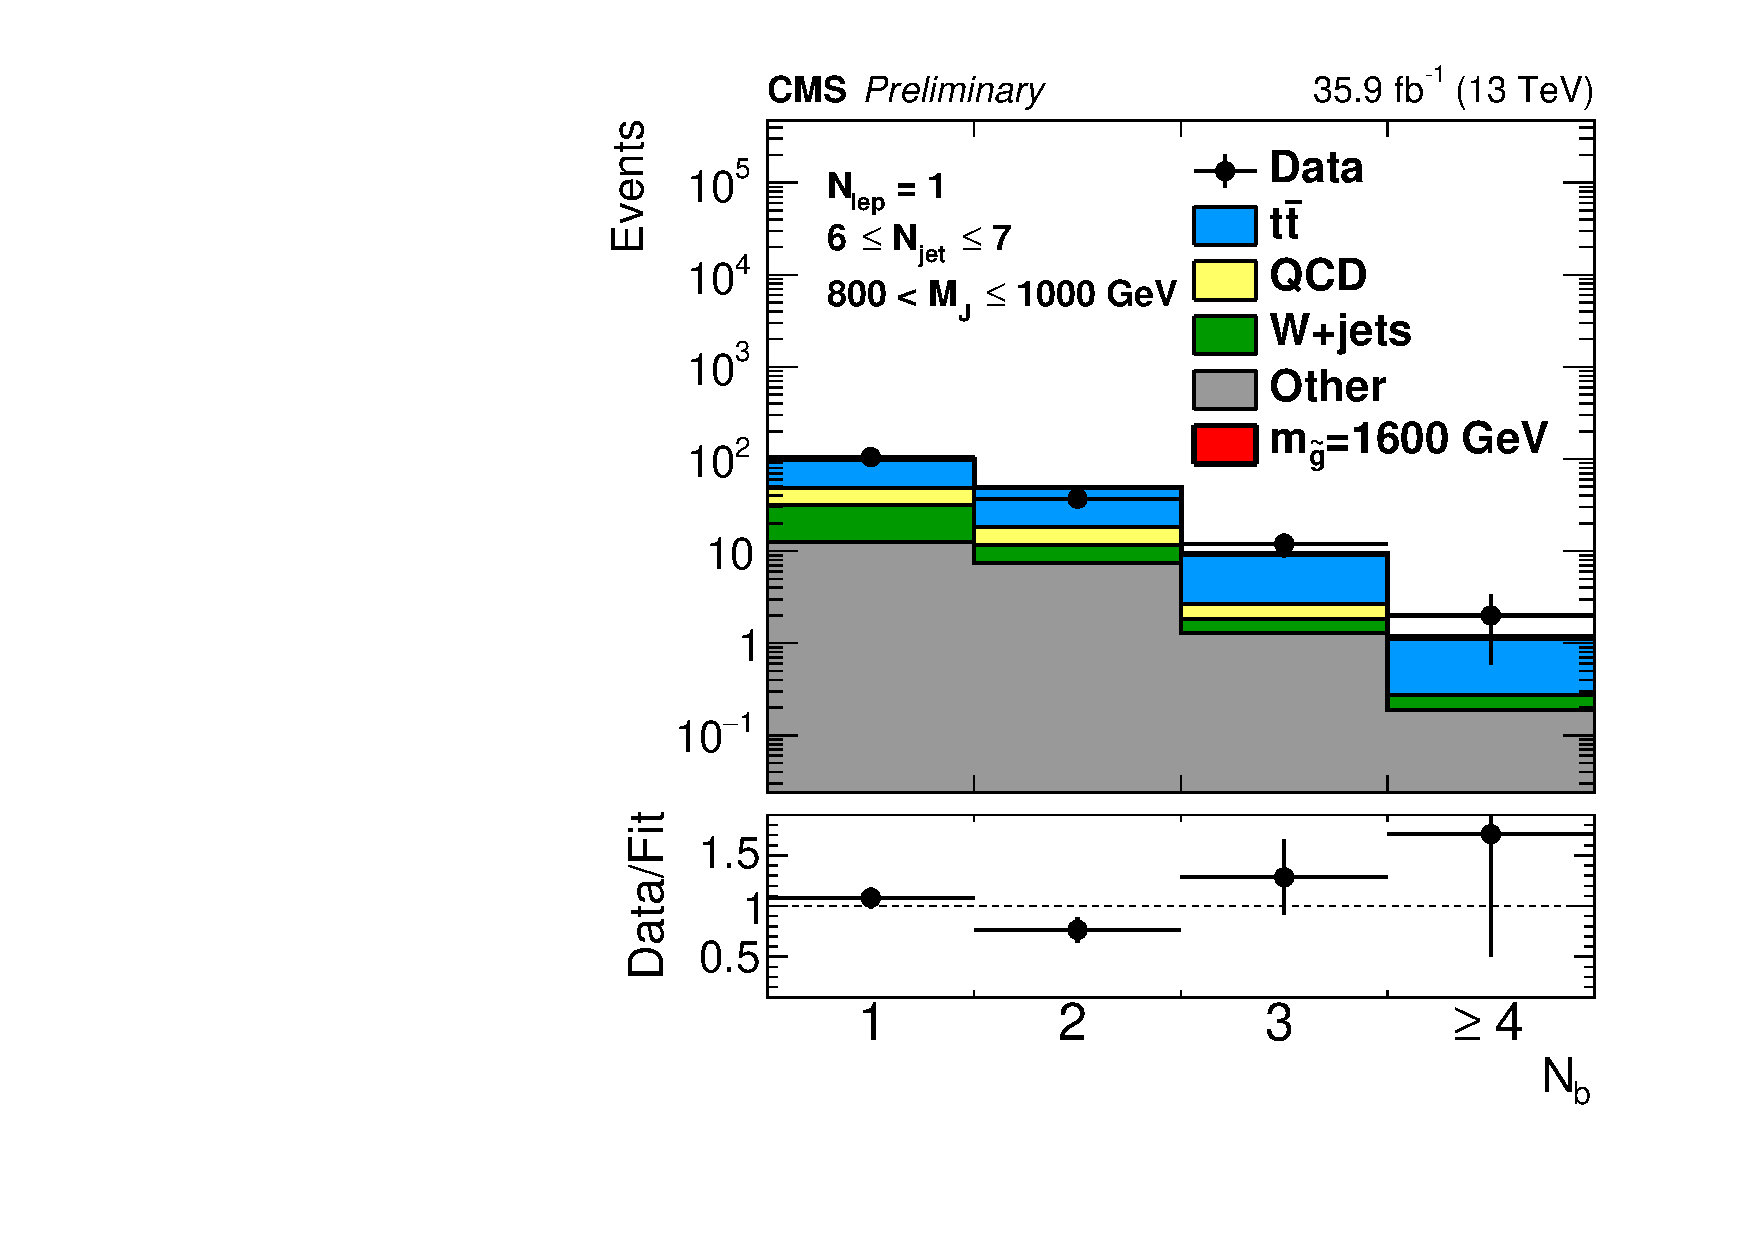
\includegraphics[angle=0,width=0.32\columnwidth]{fig/splusb_nlep1_nj67_highmj.pdf}
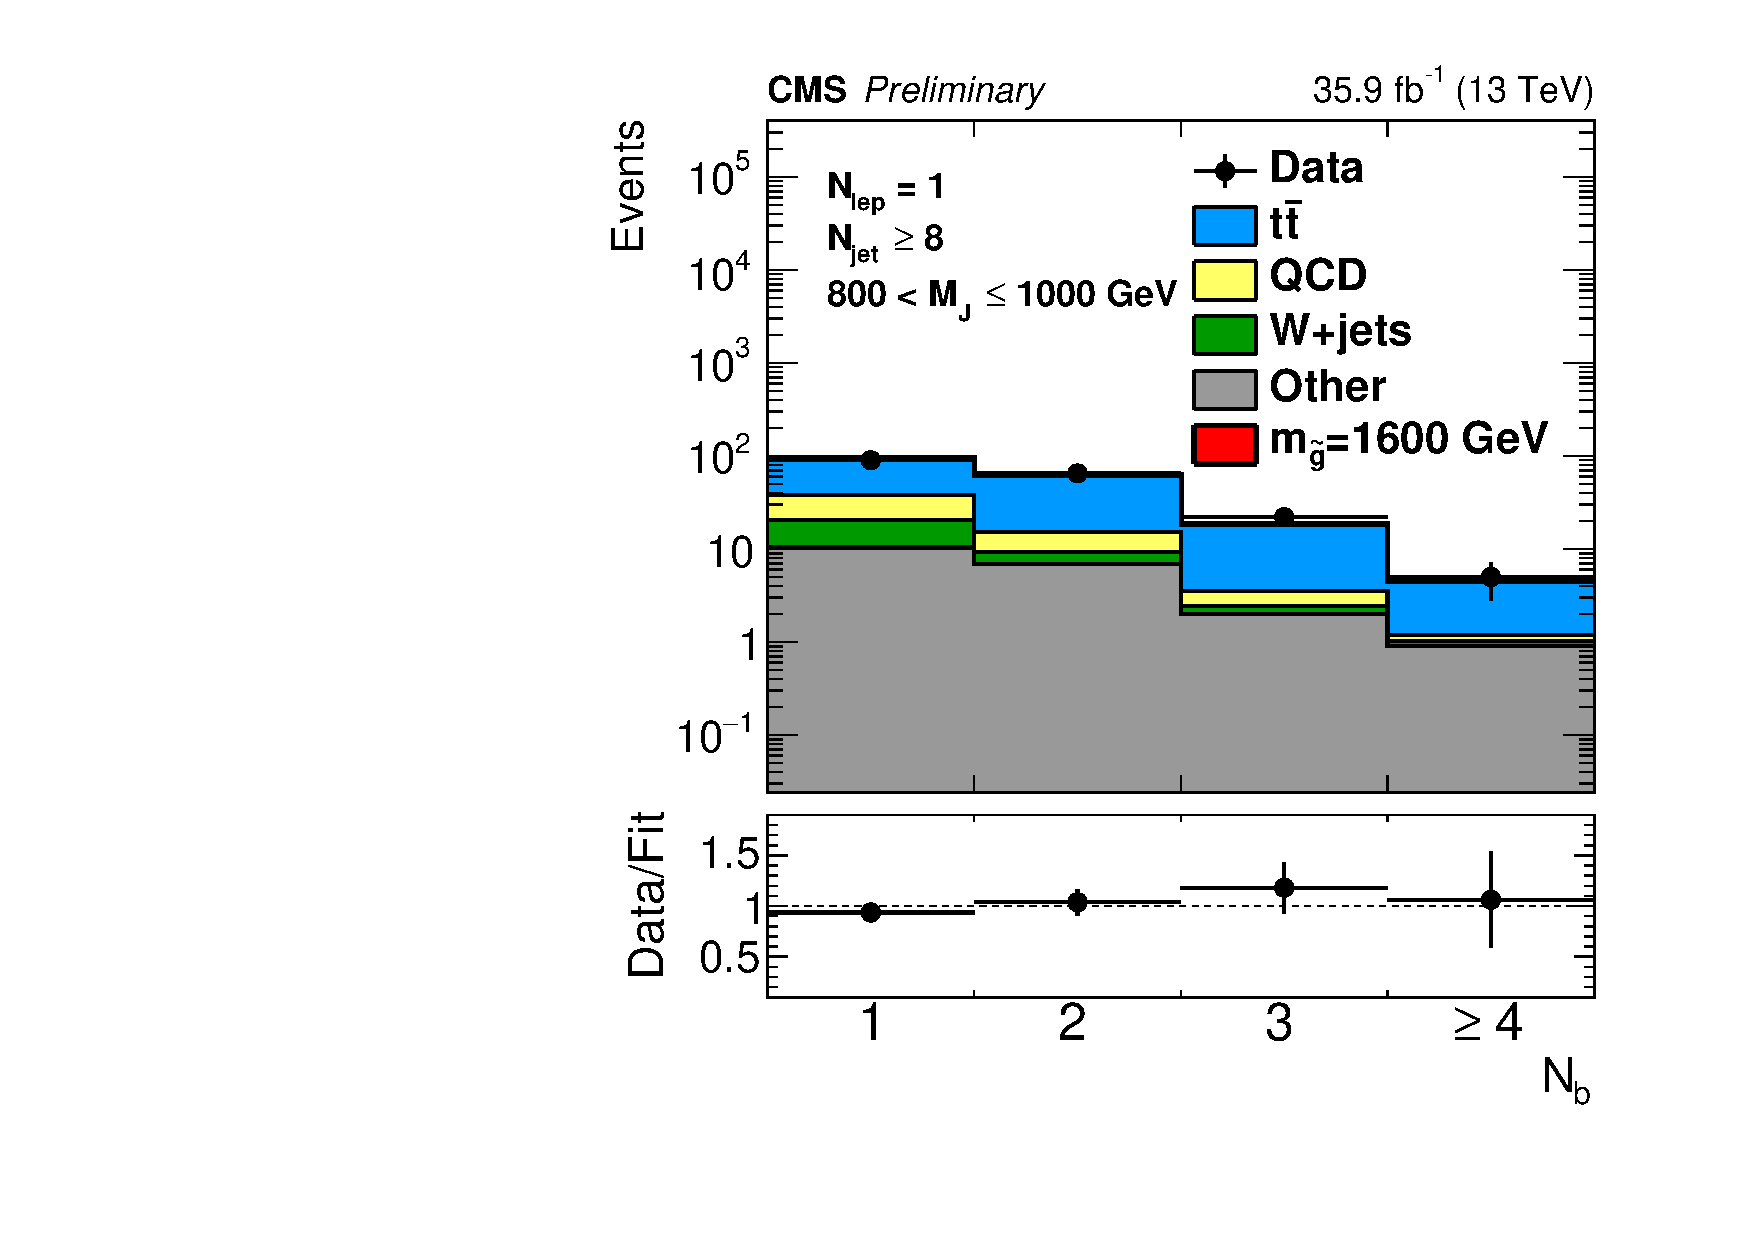
\includegraphics[angle=0,width=0.32\columnwidth]{fig/splusb_nlep1_nj8_highmj.pdf}
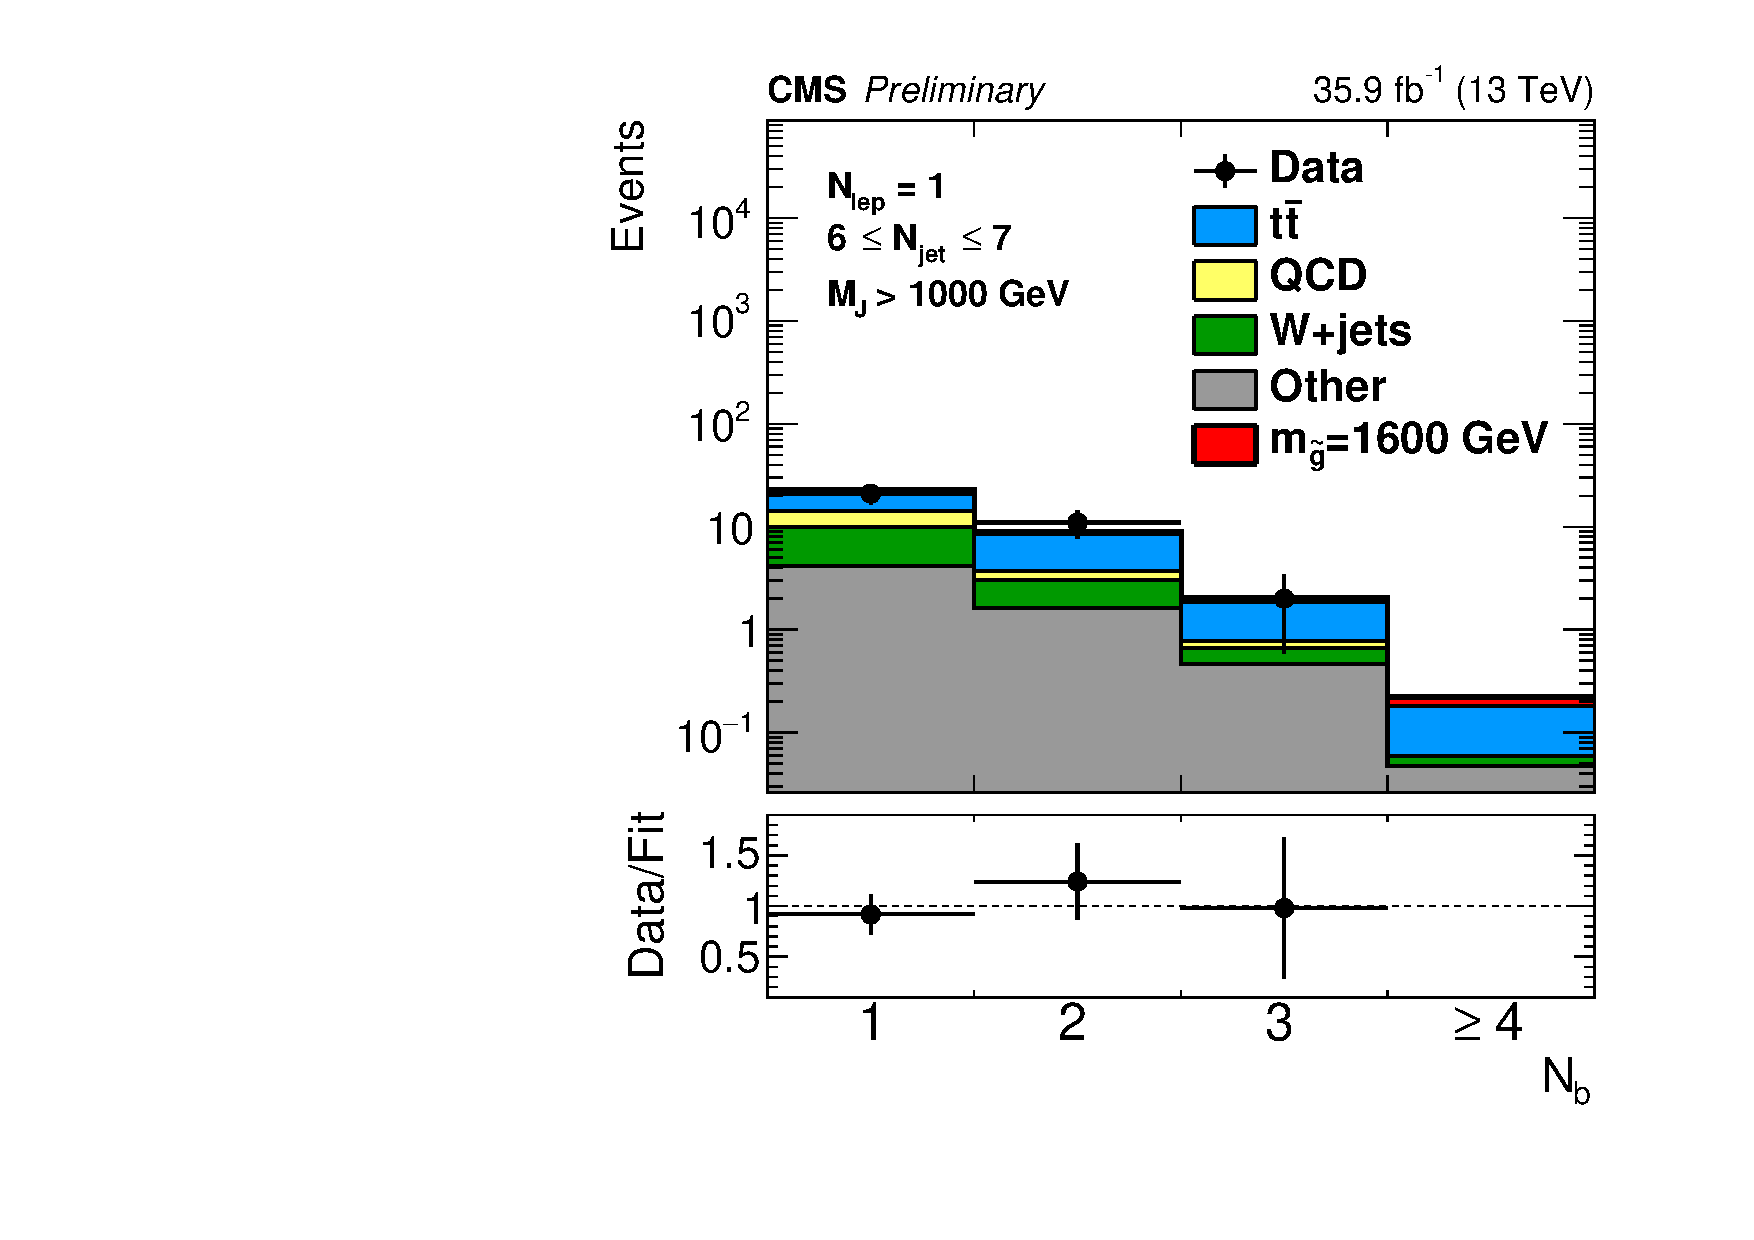
\includegraphics[angle=0,width=0.32\columnwidth]{fig/splusb_nlep1_nj67_vhighmj.pdf}
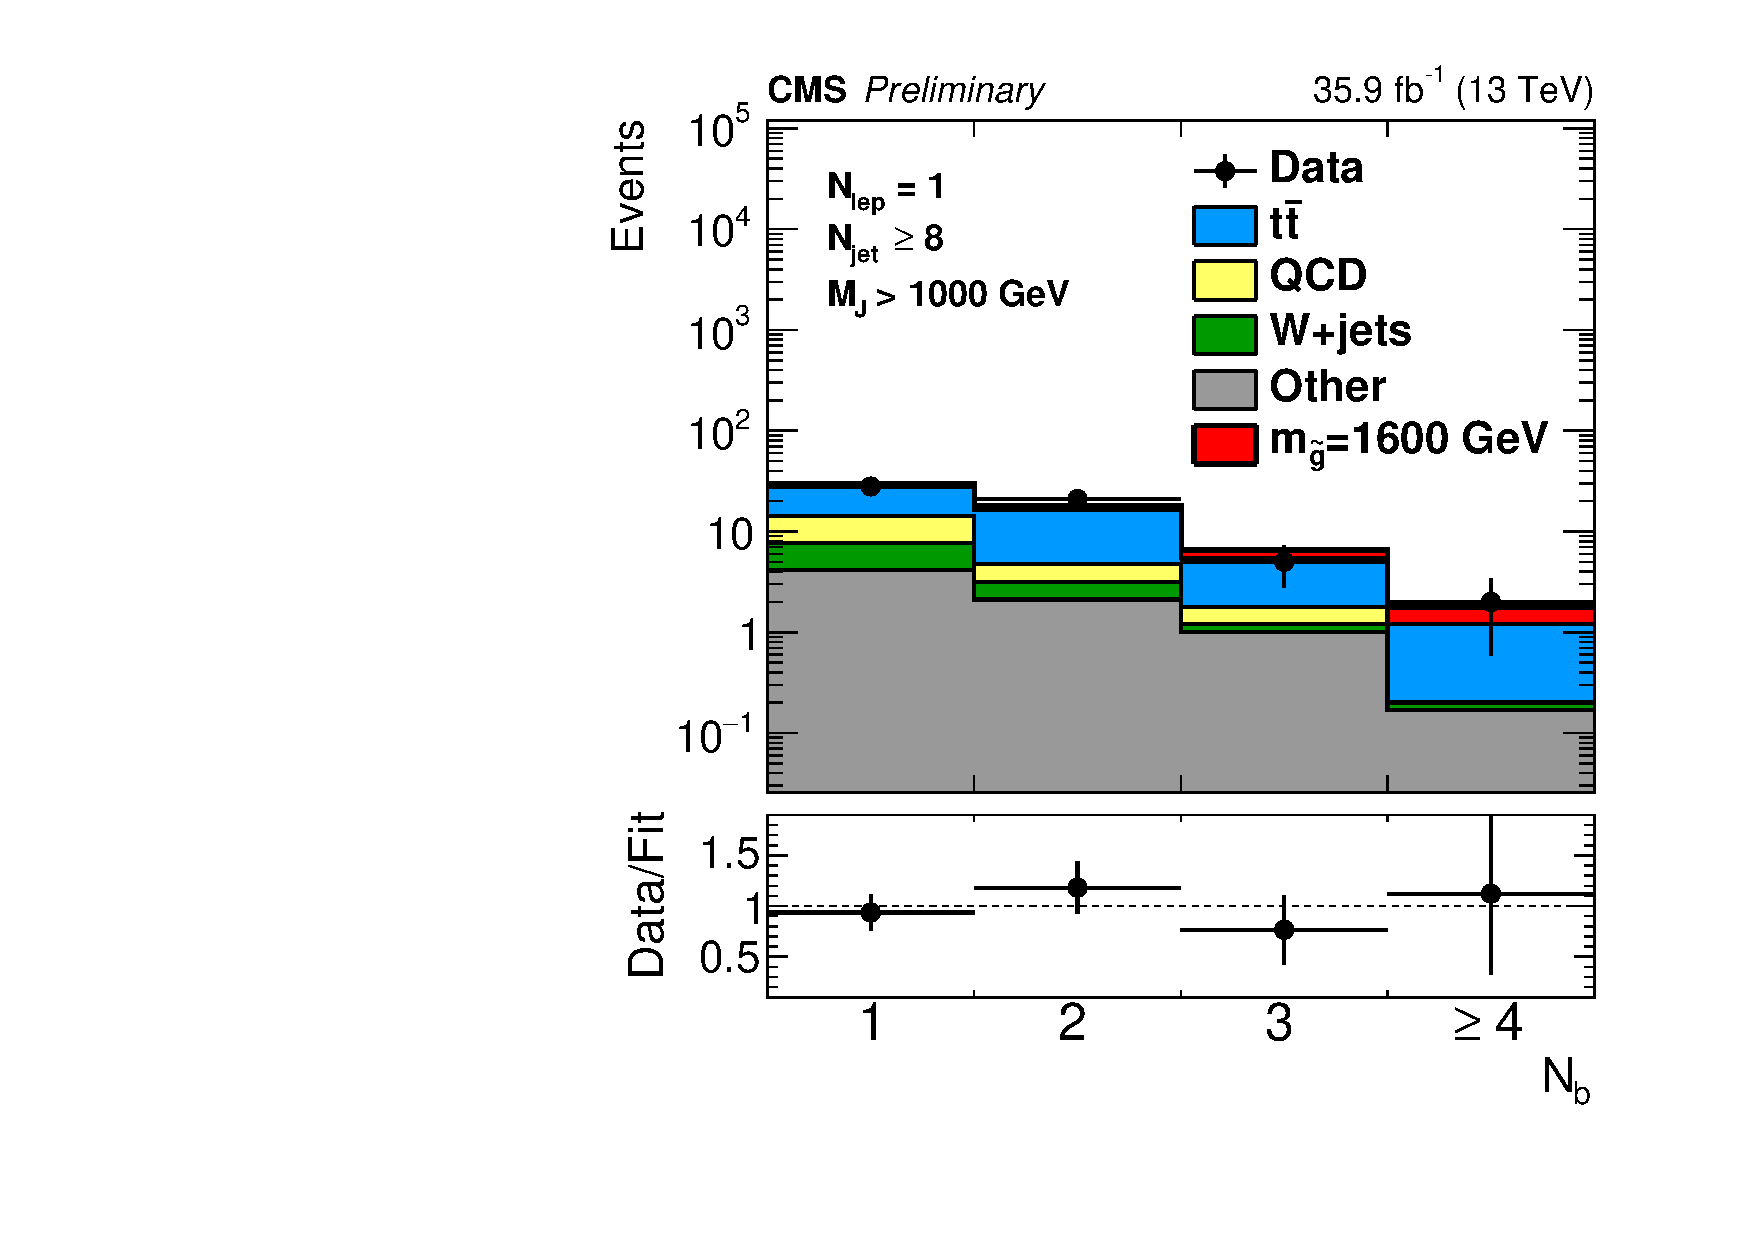
\includegraphics[angle=0,width=0.32\columnwidth]{fig/splusb_nlep1_nj8_vhighmj.pdf}
\caption{Data and the $\mglu = 1600~\GeV$ signal-plus-background post-fit \Nb distribution for the signal region bins: $\Njets \geq 8$, $500 < \MJ \leq 800~\GeV$ (upper-left), $6 \leq \Njets \leq 7$, $800 < \MJ \leq 1000~\GeV$ (upper-middle), $\Njets \geq 8$, $800 < \MJ \leq 1000~\GeV$ (upper-right), $ 6 \leq \Njets \leq 7$, $\MJ > 1000~\GeV$ (bottom-left), and $ \Njets \geq 8$, $\MJ > 1000~\GeV$ (bottom-right).
The ratio of data to post-fit yields is shown in the lower panel.
The post-fit uncertainty is depicted as a hatched band.}
\label{fig:splusb_sr}
\end{figure}

\begin{table}[tbp!]
\begin{center}
\begin{tabular}{|l|c|c|c|} \hline
                                                  &  Post-fit pull   &  Post-fit pull  &                         \\
Nuisance parameter                                &  ($b$-only fit)  &  ($s+b$ fit)    & $\rho(\theta_{i}, \mu)$ \\  
\hline
b,c jet b-tag SF (btag\_bc)                       &  +0.14, 0.93     &  +0.12, 0.94    &  -0.09                  \\
u,d,s,g jet b-tag SF (btag\_udsg)                 &  +0.25, 0.91     &  +0.22, 0.91    &  -0.05                  \\
Gluon splitting (gs)                              &  +0.50, 0.69     &  +0.45, 0.70    &  -0.14                  \\
Jet energy resolution (jer)                       &  -0.01, 0.76     &  -0.02, 0.73    &  -0.01                  \\
Jet energy scale (jes)                            &  +0.03, 0.53     &  +0.01, 0.41    &  -0.06                  \\
Lepton efficiency (lep\_eff)                      &  +0.02, 1.00     &  +0.02, 1.00    &  +0.02                  \\
Luminosity (lumi)                                 &  -0.02, 0.99     &  -0.02, 0.99    &  -0.02                  \\
Fact. scale for Other (other\_muf)                &  +0.05, 0.97     &  +0.04, 0.97    &  -0.00                  \\
Renorm. scale for Other (other\_mur)              &  +0.03, 1.09     &  +0.04, 1.09    &  +0.00                  \\
Renorm. and Fact. scale for Other (other\_murf)   &  +0.11, 0.96     &  +0.09, 0.94    &  -0.00                  \\
QCD fake rate (qcd\_fakerate)                     &  -0.12, 0.98     &  -0.10, 0.99    &  +0.03                  \\
Fact. scale for QCD (qcd\_muf)                    &  -0.05, 1.01     &  -0.05, 1.01    &  +0.00                  \\
Renorm. scale for QCD (qcd\_mur)                  &  +0.00, 0.99     &  +0.00, 0.99    &  +0.00                  \\
Renorm. and Fact. scale for QCD (qcd\_murf)       &  -0.04, 1.01     &  -0.04, 1.01    &  +0.00                  \\
Fact. scale for \ttbar (ttbar\_muf)               &  -0.03, 1.02     &  -0.03, 1.02    &  +0.00                  \\
Renorm. scale for \ttbar (ttbar\_mur)             &  +0.01, 0.99     &  +0.01, 0.98    &  +0.00                  \\
Renorm. and Fact. scale for \ttbar (ttbar\_murf)  &  -0.02, 1.01     &  -0.02, 1.01    &  +0.00                  \\
Fact. scale for \Wjets (wjets\_muf)               &  -0.00, 1.00     &  -0.00, 1.00    &  +0.00                  \\
Renorm. scale for \Wjets (wjets\_mur)             &  +0.00, 1.00     &  +0.00, 1.00    &  -0.00                  \\
Renorm. and Fact. scale for \Wjets (wjets\_murf)  &  -0.00, 1.00     &  -0.00, 1.00    &  +0.00                  \\
\hline
\end{tabular}
\caption{Table of post-fit pulls of the background-only and signal-plus-background fit.
The last column, $\rho(\theta_{i}, \mu)$, lists the correlation between the corresponding nuisance parameter, $\theta_{i}$, and the nuisance parameter controlling the signal strength, $\mu$.}
\label{tab:fit_pulls}
\end{center}
\end{table}

\end{subsection}

\end{section}

\begin{section}{Statistical Interpretation}

In the absence of significant evidence of signal, limits on the production cross section of a model can be set through the \CLs procedure~\cite{0954-3899-28-10-313,CMS-NOTE-2011-005,Junk:1999kv}.
The procedure is given by the following steps:

First, construct likelihood functions for the background-only and signal-plus-background, which for this search corresponds to the likelihood presented in Section~\ref{sec:fit_model}.

Next, in order to evaluate the compatability of the observed data with the background-only and signal-plus-background hypotheses, a test statistic, \qu, is defined as,
\begin{align}
\qu = -2\ln \frac{\mathcal{L}(N_{obs}|\mu,\hat{\theta}_{\mu})}{\mathcal{L}(N_{obs}|\hat{\mu},\hat{\theta})}, \quad  0 \leq \hat{\mu} \leq \mu
\end{align}
Here, $N_{obs}$ is the observed data, $\mu$ is the signal strength, $\theta$ represents the full set of nuisance parameters.
Additionally, $\hat{\theta}_{\mu}$ is the value of $\theta$ that maximzes the likelihood conditioned on a specified value of $\mu$, i.e. for a fixed signal strength, while $\hat{\mu}$ and $\hat{\theta}$ respectively correspond to the values of $\mu$ and $\theta$ that globally maximize the likelihood.
The structure of \qu as a likelihood ratio is motivated by the Neyman-Pearson lemma~\cite{Neyman289}, which states that the ratio of likelihoods is the most powerful discriminator.
The lower constraint of $0 \leq \hat{\mu}$ is imposed on the physical consideration that the signal cannot contribute a negative event yield, while the upper constraint of $\hat{\mu} \leq \mu$ is imposed so that upward fluctuations that result in $\hat{\mu} > \mu$ cannot be interpreted as evidence against the signal-plus-background hypothesis.

For some choice of signal strength, $\mu'$, and the observed data, calculate the observed value of $q^{obs}_{\mu'}$.

Then compute the values $\theta^{obs}_{0}$ and $\theta^{obs}_{\mu'}$, which are the values of nuisance parameters that maximize the background-only ($\mu = 0$) and signal-plus-background ($\mu = \mu'$) likelihoods under the observed data, respectively.

From the values of $\theta^{obs}_{0}$ and $\theta^{obs}_{\mu'}$, construct the probability density functions (pdfs) for $q_{\mu'}$ under the background-only hypothesis, $f(\qu|0,\theta^{obs}_{0})$, and under the signal-plus-background with $\mu'$, $f(\qu|\mu',\theta^{obs}_{\mu'})$.
These pdfs can either be determined by generating and fitting psuedoexperiments or by using asymptotic formulae for approximating the distribution of \qu~\cite{Cowan:2010js}.
The latter option is chosen, as with the former method, the computational time and power needed for generating pseudoexperiemnts for each signal mass point can be prohibitive.

Using these distributions, one can calculate the probability of observing data at least as extreme as $q^{obs}_{\mu'}$ under the backround hypothesis, \CLb, and under the signal-plus-background hypothesis, \CLsb.
Formally,
\begin{align}
\CLb = P(\qu \geq q^{obs}_{\mu'}|b) = \int^{\infty}_{q^{obs}_{0}} f(\qu|0,\theta^{obs}_{0}) d\qu,
\end{align}
and
\begin{align}
\CLsb = P(\qu \geq q^{obs}_{\mu'}|\mu's+b) = \int^{\infty}_{q^{obs}_{\mu'}} f(\qu|\mu',\theta^{obs}_{\mu'}) d\qu.
\end{align}
\end{section}
Finally, the \CLs quantity can be calculated as the ratio of these two probabilities, with
\begin{align}
\CLs(\mu) = \frac{\CLsb}{\CLb}.
\end{align}

Using the \CLs quantity, a model can be said to be excluded at the ($1 - \alpha$) confidence level (CL), if for $\mu = 1$, $\CLs \leq \alpha$.
Conventions are for the 95\% CL upper limit on $\mu$ to be quoted, corresponding to $\alpha = 0.05$, in which case the value of $\mu$ can be scanned until reaching $\CLs = 0.05$.
The resulting value of $\mu$ then represents the 95\% CL upper limit on the signal strength of the model and thus on its production cross section.

\begin{section}{Limits on the T1tbs benchmark model}

The resulting 95\% upper limits on the signal production cross section from the \CLs procedure are shown in Figure~\ref{fig:limits}, which includes the expected and observed limits along with the gluino pair production cross section.
Comparing the observed limits to the gluino pair production cross section~\cite{XSecgluinogluino} indicates that gluino masses below 1610~\GeV are excluded in the benchmark \smsDecay model.
The observed limits are slightly less stringent than the expected limits, which is largely due to the insignificant excess in the $\MJ > 1000~\GeV$, $\Njets > 8$ and $\Nb \geq 4$ bin.

\begin{figure}[tbp!]
\centering
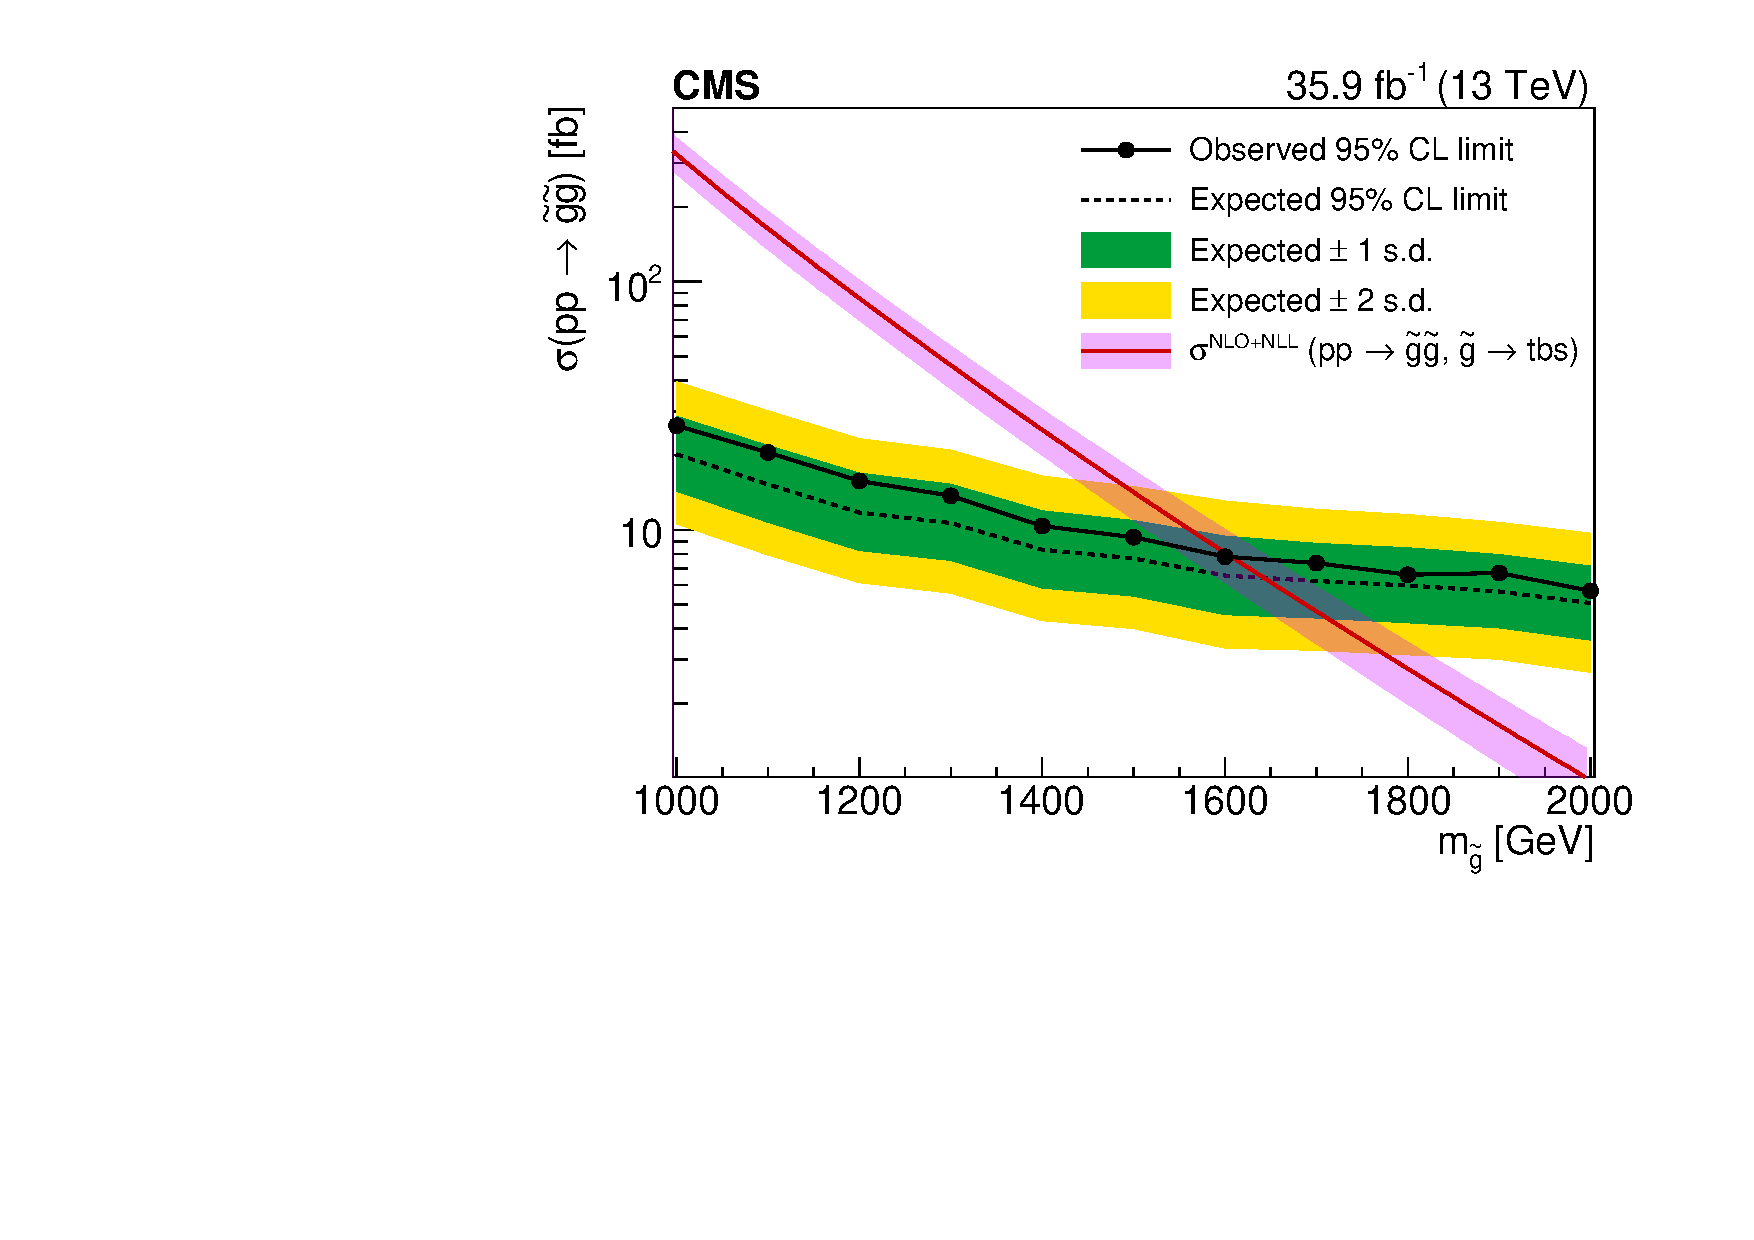
\includegraphics[angle=0,width=0.80\columnwidth]{fig/limits.pdf}
\caption{Cross section upper limits at 95\% CL for a model of gluino pair production with \smsDecay compared to the gluino pair production cross section.
The theoretical uncertainties in the cross section are shown as a band around the
red line~\cite{XSecgluinogluino}.
The expected limits (dashed line) and their $\pm1$~s.d.\ and $\pm2$~s.d.\ variations are shown as green and yellow bands, respectively.
The observed limit is shown by the solid line with dots.}
\label{fig:limits}
\end{figure}

\end{section}
